%---------------------------------------------------------------------
%
%                          main.tex
%
%---------------------------------------------------------------------
%
% main.tex
% Copyright 2015 Dr. Francisco J. Pulido
%
% This presentation belongs to the PhD titled "New Techniques and Algorithms for Multiobjective and Lexicographic Goal-Based Shortest Path Problems", distributed under the Creative Commons Licence Attribution-NonCommercial-NoDerivs 3.0, available in http://creativecommons.org/licenses/by-nc-nd/3.0/. The complete PhD dissertation is freely accessible from http://www.lcc.uma.es/~francis/

\documentclass[xcolor=dvipsnames, t]{beamer}
\usetheme{Madrid}
\usecolortheme{orchid}

\defbeamertemplate{subsection in toc}{bullets}{%
  \leavevmode
  \parbox[t]{1em}{\textbullet\hfill}%
  \parbox[t]{\dimexpr\textwidth-1em\relax}{\inserttocsubsection}\par}
\defbeamertemplate{section in toc}{sections numbered roman}{%
  \leavevmode%
  \MakeUppercase{\romannumeral\inserttocsectionnumber}.\ %
  \inserttocsection\par}

\setbeamertemplate{section in toc}[sections numbered roman]
\setbeamertemplate{subsection in toc}[bullets]

\usepackage[utf8]{inputenc}
\usepackage{fancybox}
\usepackage{framed}
\usepackage{pgfpages}

\definecolor{ao}{rgb}{0.0, 0.0, 1.0}

\newif\ifisnotes
\input{Temp}
\ifisnotes
\pgfpagesuselayout{2 on 1}[]
\setbeameroption{show notes on second screen=bottom}
\setbeamertemplate{note page}[plain]
\fi


% Commands with algorithm names and theorems
% -----------------------------------------------------------------------------
%---------------------------------------------------------------------
%
%                          commands.tex
%
%---------------------------------------------------------------------
%
% commands.tex
% Copyright 2015 Dr. Francisco J. Pulido
%
% This presentation belongs to the PhD titled "New Techniques and Algorithms for Multiobjective and Lexicographic Goal-Based Shortest Path Problems", distributed under the Creative Commons Licence Attribution-NonCommercial-NoDerivs 3.0, available in http://creativecommons.org/licenses/by-nc-nd/3.0/. The complete PhD dissertation is freely accessible from http://www.lcc.uma.es/~francis/
%
% Algorithm acronyms
%%%%%%%%%%%%%%%%%%%%%%%%%%%%%%%%%%%%%%%%%%%%%%%%%%%%%%%%%%%%%%%%%%%%%%

\def\astar{$A^*$}
\def\namoa{$\text{NAMOA}^*$}
\def\tc{$\text{TC}$}
\def\moa{$\text{MOA}^*$}
\def\metal{$\text{METAL-A}^*$}
\def\namoalex{$\text{NAMOA}^{*}_{\text{lex}}$}
\def\namoalin{$\text{NAMOA}^{*}_{\text{lin}}$}
\def\namoadr{$\text{NAMOA}^{*}_{\text{dr}}$}

\def\lexgo{$\text{LEXGO}^*$}
\def\lexgolex{$\text{LEXGO}^*_{\text{lex}}$}
\def\lexgolin{$\text{LEXGO}^*_{\text{lin}}$}
\def\lexgodr{$\text{LEXGO}^*_{\text{dr}}$}





\title[PhD Dissertation]{New Techniques and Algorithms for Multiobjective and Lexicographic Goal-Based Shortest Path Problems}
\subtitle{PhD Dissertation}

\author[Francisco J. Pulido Arrebola]{Francisco J. Pulido Arrebola \newline
{\small Supervised by: Dr. Lawrence Mandow}}

\institute[]{Dept. Lenguajes y Ciencias de la Computaci\'{o}n \\
E.T.S. Ingeniería Inform\'{a}tica \\
  Universidad de M\'alaga}

\titlegraphic{
\includegraphics[width=150px,height=45px]{figs/logos}}
  
\date{July 7, 2015}

% Document
% -----------------------------------------------------------------------------
\begin{document}

\begin{frame}[noframenumbering]
\titlepage
\end{frame}

\begin{frame}[noframenumbering]
\frametitle{Outline}
\tableofcontents[hideallsubsections]
\end{frame}

\AtBeginSection[]
{
\begin{frame}<beamer>[noframenumbering]
\frametitle{Outline}
\tableofcontents[
  currentsection,
  sectionstyle=show/show,
  subsectionstyle=show/shaded/hide
]
\end{frame}
}

\AtBeginSubsection[]
{
\begin{frame}<beamer>[noframenumbering]
\frametitle{Outline}
\tableofcontents[
  currentsection,
  sectionstyle=show/show,
  subsectionstyle=show/shaded/hide
]
\end{frame}
}

% Introduction
% -----------------------------------------------------------------------------
%---------------------------------------------------------------------
%
%                          introduction.tex
%
%---------------------------------------------------------------------
%
% introduction.tex
% Copyright 2015 Dr. Francisco J. Pulido
%
% This presentation belongs to the PhD titled "New Techniques and Algorithms for Multiobjective and Lexicographic Goal-Based Shortest Path Problems", distributed under the Creative Commons Licence Attribution-NonCommercial-NoDerivs 3.0, available in http://creativecommons.org/licenses/by-nc-nd/3.0/. The complete PhD dissertation is freely accessible from http://www.lcc.uma.es/~francis/

\section{Introduction}

\subsection{Motivation}

\begin{frame} 
\frametitle{The Shortest Path Problem (SPP)}
	\begin{block}{Definition}
		The SPP consists in finding a minimal cost path between two nodes in a graph, where the graph is composed of arcs labeled with the cost of the transition between nodes.
	\end{block}
	\begin{itemize}
		\item Solved by Dijkstra in 1959 and by Hart et al. (\astar) in 1968 exploiting specific problem knowledge.
	\end{itemize}
\begin{columns}%[onlytextwidth, t]
\column{0.35\linewidth}
    \begin{block}{Research fields}<2>
    	\begin{itemize}
		\item Artificial Intelligence
		\item Operational Research
		\end{itemize}
    \end{block}
\column{0.45\linewidth}
    \begin{figure}
    \centering
    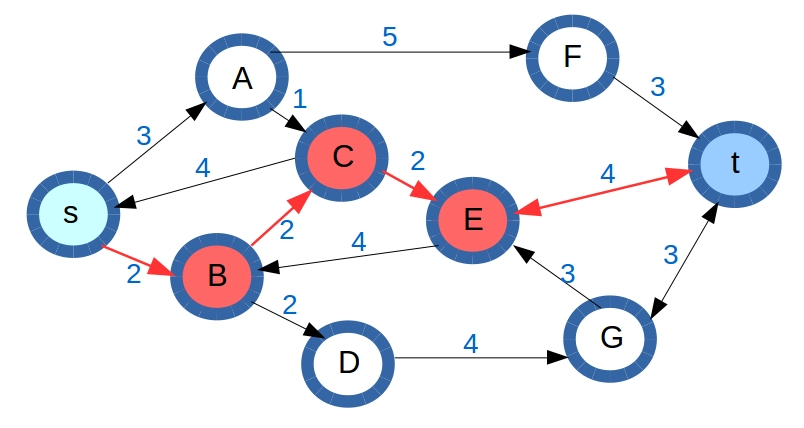
\includegraphics[scale=0.25]{figs/spp}
  \end{figure}
\end{columns}     
\note{The introduction of this thesis begins with the shortest path problem. Given a problem that can be modeled as a graph with nodes representing different states of the problem and the arcs the cost of the transition between those states, the Shortest Path problem is the problem of finding the route with minimal cost between two given nodes, the start and the target nodes.

The Dutch computer scientist Dijkstra in 1959 presented the first algorithm to solve this problem and Hart et al. in 1968 presented \astar, the first optimal algorithm to solve the problem by using specific knowledge acquired from the problem to be solved. Since then, the shortest path problem has been one of the most studied problems in the Artificial Intelligence and Operational Research fields}
\end{frame}
%%%%%%%%%%%%%%%%%%%%%%%%%%%%%%%%%%%%%%%%%%%%%%%%%%%%%%%%%%%%%%%%%%%%%%%%%%%%%%%%%%%%%%%%%%%%%%%%%%%%%%%%%
\begin{frame}[t]  
\frametitle{Applications to the SPP}
  \begin{itemize}
  	\item Path planning in game maps.
  	\vspace{2mm}
  	\begin{itemize}
  		\item The game map is represented as a graph.
  		 \vspace{2mm}
  		\item The characters movement through the map is solved as a SPP.
  	\end{itemize}
  \end{itemize}
  \vspace{4mm}
  \begin{center}
    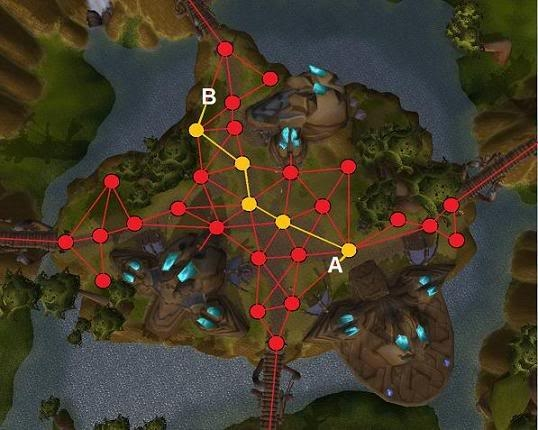
\includegraphics[scale=0.4]{figs/game_maps}
  \end{center}
  \note{One of the typical applications for the SPP is path planning in game maps. As we see in this picture, the possible movements of the characters within the map are represented as a graph.}
\end{frame}
%%%%%%%%%%%%%%%%%%%%%%%%%%%%%%%%%%%%%%%%%%%%%%%%%%%%%%%%%%%%%%%%%%%%%%%%%%%%%%%%%%%%%%%%%%%%%%%%%%%%%%%%%
\begin{frame}[t] 
\frametitle{Applications to the SPP}
  \begin{itemize}
  \item Motion planning in mobile robots.
  \vspace{2mm}
  \begin{itemize}
  		\item The terrain is represented as a graph.
  		\vspace{2mm}
  		\item The robot must find a path avoiding obstacles.
  	\end{itemize}
  \end{itemize}
  \vspace{4mm}  
  \begin{center}
    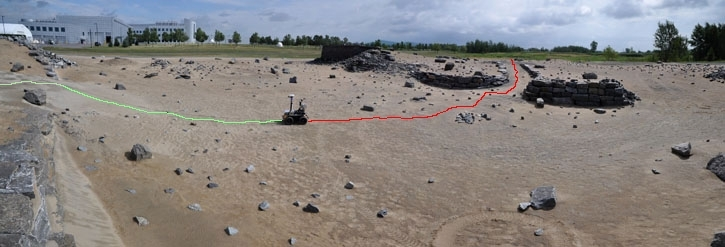
\includegraphics[scale=0.5]{figs/robot}
  \end{center}
  \note{Another application for the SPP is motion planning in mobile robots, where the terrain represents the graph that the robot traverses avoiding the obstacles.}
\end{frame}
%%%%%%%%%%%%%%%%%%%%%%%%%%%%%%%%%%%%%%%%%%%%%%%%%%%%%%%%%%%%%%%%%%%%%%%%%%%%%%%%%%%%%%%%%%%%%%%%%%%%%%%%%
\begin{frame}[t]  
\frametitle{Applications to the SPP}
  \begin{itemize}
  \item Route planning in road maps.
  \vspace{2mm}
  \begin{itemize}
  		\item Real road networks are graphs.
  		\vspace{2mm}
  		\item Arcs represent road junctions.
  		\vspace{2mm}
  		\item Arcs are typically labeled with the distance between junctions.
  	\end{itemize}
  \end{itemize}
  \vspace{3mm}
  \begin{center}
    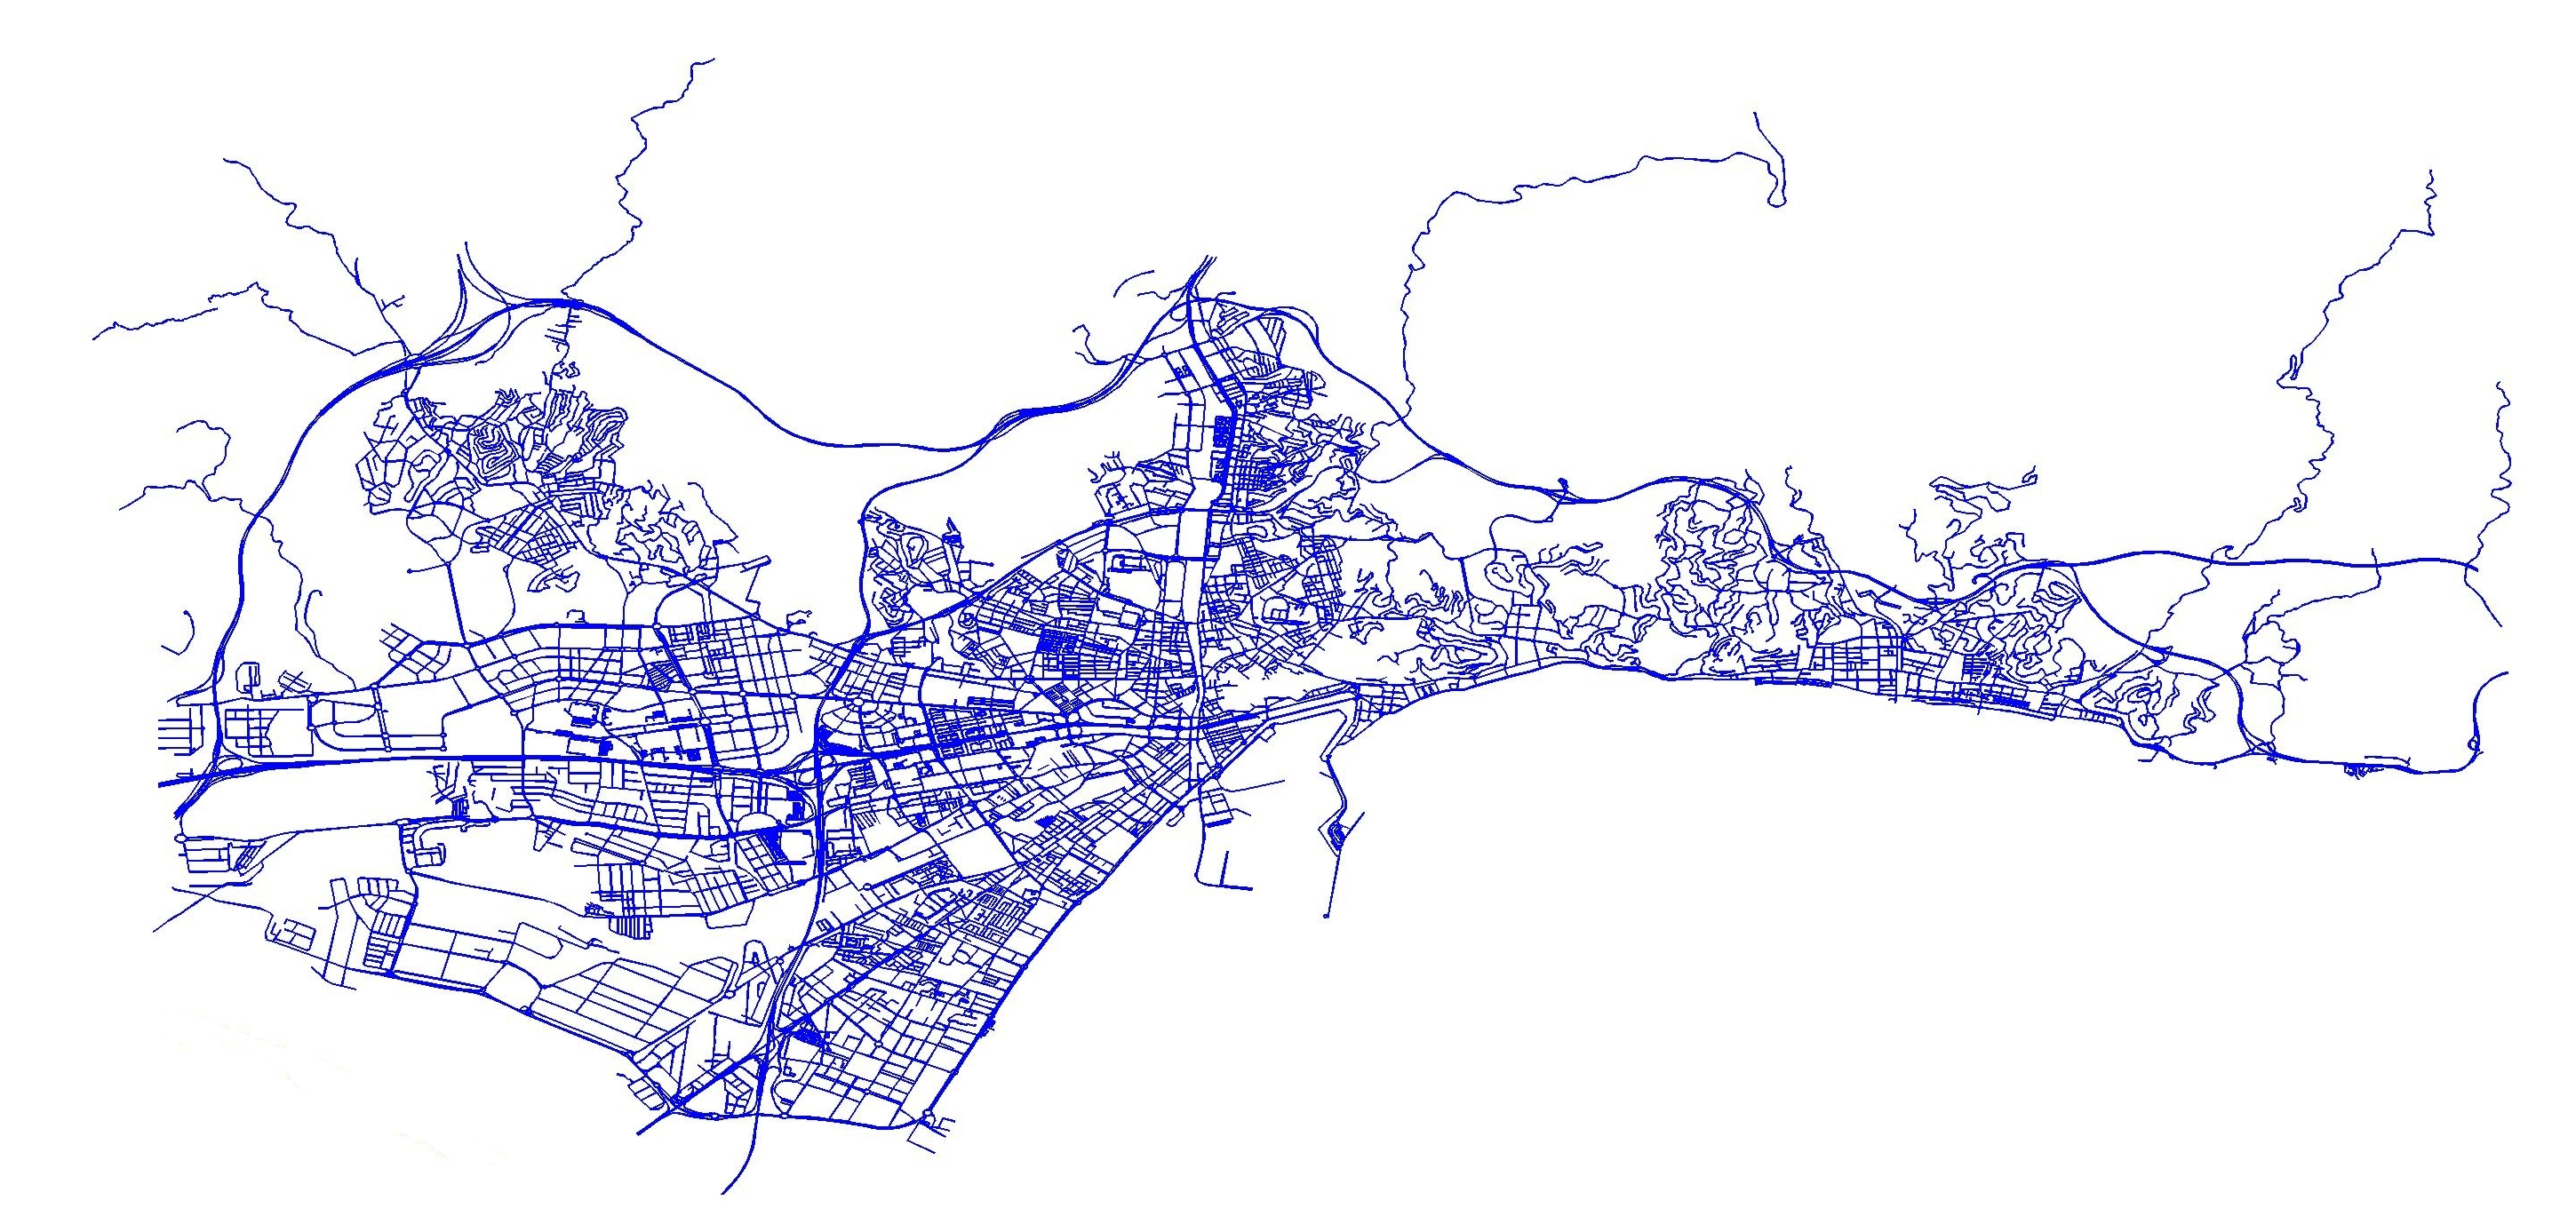
\includegraphics[scale=0.125]{figs/malaga_map}
  \end{center}
  \note{And, perhaps, the route planning in road networks is one of the most natural and studied applications of the shortest path problem. We use in our daily basis google maps or GPS devices to help us plan our trips, and find for us the shortest route to our destination.}
\end{frame}
%%%%%%%%%%%%%%%%%%%%%%%%%%%%%%%%%%%%%%%%%%%%%%%%%%%%%%%%%%%%%%%%%%%%%%%%%%%%%%%%%%%%%%%%%%%%%%%%%%%%%%%%%
\begin{frame} 
\frametitle{Multicriteria Search Problem (MSP)}
	\begin{block}<1->{Definition}
  		\vspace{1mm}
		MSP is the natural extension of SPP to the multicriteria case, where arcs are labeled with \textcolor{ao}{vectors} instead of scalar values.
		\vspace{1mm}	
	\end{block}
	\vspace{8mm}
	\begin{columns}[onlytextwidth, t]
	\column{0.3\linewidth}
	SPP \\
	\vspace{5mm}
	Decision problems 
	\column{0.1\linewidth}
	$\longrightarrow$ \\
	\vspace{5mm}
	$\longrightarrow$ \\	
	\column{0.5\linewidth}
	single-objective optimization problem \\
	\vspace{5mm}
	multiple conflicting criteria
	\end{columns}
\note{SPP has been traditionally considered a single-objective optimization problem. Real decision problems \qquad $\longrightarrow$ \qquad frequently involve multiple conflicting criteria. What is the Multicriteria Search Problem? It's the natural extension of the Shortest Path Problem when several criteria are taken into account simultaneously. The solution to this problem is no longer a single optimal value, but a set of non-dominated or Pareto-optimal paths. We will get deeper into this concept in the following slides, but let's first talk about human decisions.
IMP: Decisions are taken by humans}
\end{frame}
%%%%%%%%%%%%%%%%%%%%%%%%%%%%%%%%%%%%%%%%%%%%%%%%%%%%%%%%%%%%%%%%%%%%%%%%%%%%%%%%%%%%%%%%%%%%%%%%%%%%%%%%%
\begin{frame} 
\frametitle{Human decisions}
	Humans make choices according to their personal preferences, which involve simultaneously multiple, and often, conflicting criteria.
	\vspace{3mm}
	\begin{columns}[onlytextwidth, t]
\column{0.7\linewidth}
	\begin{center}
		
\includegraphics[scale=0.25]{figs/decision}
	\end{center}
\column{0.3\linewidth}
	\only<2->{New car?}
	\begin{itemize}
		\item<2-> Price
		\item<2-> Speed
		\item<2-> Brand
		\item<2-> Color
	\end{itemize}	
	\vspace{3mm}
	\only<3->{A route home?}
	\begin{itemize}
		\item<3-> Distance?
	\end{itemize}
\end{columns} 	

\note{How do we make decisions? We are complex, that's certain, and we make decisions considering multiple criteria, that's certain too. If I'm going to buy a new car, I will consider the price, speed, brand, color... and if I'm checking my GPS device and it is presented to me the shortest route ... it seems that something is missing, isn't it?}
\end{frame}
%%%%%%%%%%%%%%%%%%%%%%%%%%%%%%%%%%%%%%%%%%%%%%%%%%%%%%%%%%%%%%%%%%%%%%%%%%%%%%%%%%%%%%%%%%%%%%%%%%%%%%%%%
\begin{frame} 
\frametitle{Route planning in road maps}
  	\begin{center}
		\includegraphics<1>[scale=0.25]{figs/2}
		\includegraphics<2>[scale=0.25]{figs/3}
		\includegraphics<3>[scale=0.25]{figs/4}
		\includegraphics<4>[scale=0.25]{figs/5}
		\includegraphics<5>[scale=0.25]{figs/6}
		\includegraphics<6>[scale=0.25]{figs/7}
		\includegraphics<7>[scale=0.25]{figs/8}
		\includegraphics<8>[scale=0.25]{figs/9}
	\end{center}
		\note{Let me now present an example of a typical route planning problem. I have finished an important meeting and I will use my fantastic route planning application to find me the shortest path back home.\\
The length of the shortest path from all possible routes is 90 km.\\
Wait! There's a traffic jam on that route and the travel time would be an hour and a half.\\
Maybe, what I do want is not the shortest but the fastest route.\\
This route is 10 kms longer but half an hour faster, it seems to me a good trade-off.\\
or not, there's a toll and this route is 8 euros more expensive than the last.\\
What about a cheaper route?\\
Well, this one is 20 kms longer than the first alternative, 10 minutes slower than the second, but cheaper.}
\end{frame}
%%%%%%%%%%%%%%%%%%%%%%%%%%%%%%%%%%%%%%%%%%%%%%%%%%%%%%%%%%%%%%%%%%%%%%%%%%%%%%%%%%%%%%%%%%%%%%%%%%%%%%%%%
\begin{frame} 
\frametitle{Multicriteria Search Problem (MSP)}
	\begin{block}{Definition}
		\vspace{1mm}
		\textbf{Dominance} or Pareto preference $\prec$: \\
		\begin{center}
		$ \vec{y} \prec \vec{y'} \quad
		\Leftrightarrow \quad
		\forall i \ (1\leq~i\leq~q) \quad y_i \leq y'_i \ \land \ \vec{y} \neq \vec{y'} $ \\
		\vspace{3mm}
		where $ \vec{y} = (y_1, y_2, ..., y_q)$ represents a solution path in the cost space.
		\end{center}
	\end{block}
	\vspace{4mm}
	\begin{example}
		Route cost representation: $\vec{y} = (y_1, y_2, y_3) \ \rightarrow \ \vec{y} = (120, 70, 15)$	
	\end{example}
\note{}
\end{frame}
%%%%%%%%%%%%%%%%%%%%%%%%%%%%%%%%%%%%%%%%%%%%%%%%%%%%%%%%%%%%%%%%%%%%%%%%%%%%%%%%%%%%%%%%%%%%%%%%%%%%%%%%%
\begin{frame}
\frametitle{Pareto optimality}
	\begin{center}
		\includegraphics<1>[scale=0.5]{figs/pareto1}
		\includegraphics<2>[scale=0.5]{figs/pareto2}
	\end{center}
\note{
}
\end{frame}
%%%%%%%%%%%%%%%%%%%%%%%%%%%%%%%%%%%%%%%%%%%%%%%%%%%%%%%%%%%%%%%%%%%%%%%%%%%%%%%%%%%%%%%%%%%%%%%%%%%%%%%%%
\begin{frame} 
\frametitle{Multicriteria Search Problem (MSP)}
	\begin{block}{Definition}
		\vspace{1mm}
		The solution to a MSP, \textcolor{red}{without any knowledge of the user preferences}, is the set of \textcolor{ao}{non-dominated} solution paths, or \textcolor{ao}{Pareto frontier}.
		\vspace{1mm}
	\end{block}
\note{}
\end{frame}
%%%%%%%%%%%%%%%%%%%%%%%%%%%%%%%%%%%%%%%%%%%%%%%%%%%%%%%%%%%%%%%%%%%%%%%%%%%%%%%%%%%%%%%%%%%%%%%%%%%%%%%%%
\begin{frame}
\frametitle{Pareto optimality}
	\begin{center}
		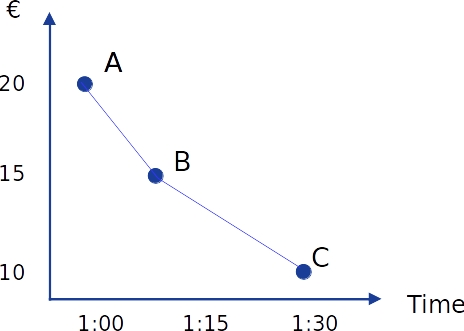
\includegraphics[scale=0.5]{figs/pareto3}
	\end{center}
\note{
}
\end{frame}
%%%%%%%%%%%%%%%%%%%%%%%%%%%%%%%%%%%%%%%%%%%%%%%%%%%%%%%%%%%%%%%%%%%%%%%%%%%%%%%%%%%%%%%%%%%%%%%%%%%%%%%%%
\begin{frame} 
\frametitle{Goal Programming}
	\begin{block}{Definition}
	\vspace{1mm}
		Goal Programming (GP) is one of the \textcolor{ao}{most successful techniques} to solve multicriteria problems. It is also a \textcolor{ao}{natural way to express user preferences} as targets or aspiration levels: $y_i \leq t_i$.
	\vspace{1mm}	
	\end{block}
	\vspace{2mm}
	\begin{block}{Definition}
	\vspace{1mm}
		Lexicographic Goal Programming (LGP) \textcolor{ao}{ranks all goals in order of importance}, dividing them into lexicographic levels of importance.
	\vspace{1mm}
	\end{block}
	\vspace{2mm}
	\begin{block}{Definition}
	\vspace{1mm}
		The deviation from a goal in a minimization problem represents a \textcolor{ao}{positive distance} between the i-th goal and its aspiration level: $d_i = \max(0, y_i - t_i)$.
	\vspace{1mm}
	\end{block}
\note{}
\end{frame}
%%%%%%%%%%%%%%%%%%%%%%%%%%%%%%%%%%%%%%%%%%%%%%%%%%%%%%%%%%%%%%%%%%%%%%%%%%%%%%%%%%%%%%%%%%%%%%%%%%%%%%%%%
\begin{frame}
\frametitle{Goal Programming}
	\begin{example}
		Three criteria (economic cost (euros), travel time (minutes), and distance (km)) grouped in \textcolor{ao}{two priority levels} where level 1 is \textcolor{ao}{infinitely more important} than level 2. The importance of the criteria within a level is defined by \textcolor{ao}{weights} as: 
	\end{example}
	\begin{equation*}
     \begin{array}{cll}
     	\textrm{Level 1:} & cost \leq 15,      & w_1 = 0.5 \\
     					  & time \leq 75 ,     & w_2 = 0.5 \\ 
       	\textrm{Level 2:} & distance \leq 120, & w_3 = 1.
     \end{array}
   \end{equation*}
   \begin{example}
		Let's assume a \textcolor{ao}{solution path} with cost $\vec y = (10, 60, 150)$, \\
		its \textcolor{ao}{deviation} from those goals is $\vec d$ = (0, \textcolor<2>{red}{30)} $\rightarrow$ \\
		$(\max(0, (10 - 15) \times 0.5) + \max(0, (60 - 75) \times 0.5)$, \textcolor<2>{red}{$(150 - 120) \times 1$})
	\end{example}
\note{Let me assume 3 criteria grouped in two priority levels, where the first level is infinitely more important than the second. Goals 2 and 3 share the same importance within level 2. Let's see some examples of vectors and their deviation: the first one (16,16,20) does not have any deviation from goals, none of objectives have overpassed the goals. This vector, however, has deviation of 4 units in the first level. In the last example, we observe deviation in both levels.}
\end{frame}
%%%%%%%%%%%%%%%%%%%%%%%%%%%%%%%%%%%%%%%%%%%%%%%%%%%%%%%%%%%%%%%%%%%%%%%%%%%%%%%%%%%%%%%%%%%%%%%%%%%%%%%%%
\begin{frame}<beamer:0>
\frametitle{Goal Programming}
	\begin{alertblock}{Dominance in GP}
		\vspace{1mm}
		In general, GP models \textcolor{red}{do not guarantee that the solution found is non-dominated}, only that satisfies the goals. However, in this research work we \textcolor{red}{only seek for non-dominated solutions} that satisfy the goals.
		\vspace{1mm}
	\end{alertblock}
\note{}
\end{frame}
%%%%%%%%%%%%%%%%%%%%%%%%%%%%%%%%%%%%%%%%%%%%%%%%%%%%%%%%%%%%%%%%%%%%%%%%%%%%%%%%%%%%%%%%%%%%%%%%%%%%%%%%%
\begin{frame}
\frametitle{Lexicographic goals}
	\begin{center}
		\includegraphics<1>[scale=0.6]{figs/goals1}
		\includegraphics<2>[scale=0.6]{figs/extreme-solutions}
		\includegraphics<3>[scale=0.6]{figs/goals2}
		\includegraphics<4>[scale=0.6]{figs/goals3}
		\includegraphics<5>[scale=0.6]{figs/goals4}
		\includegraphics<6>[scale=0.6]{figs/goals5}
		\includegraphics<7>[scale=0.6]{figs/goals6}
	\end{center}
\note{}
\end{frame}
%%%%%%%%%%%%%%%%%%%%%%%%%%%%%%%%%%%%%%%%%%%%%%%%%%%%%%%%%%%%%%%%%%%%%%%%%%%%%%%%%%%%%%%%%%%%%%%%%%%%%%%%%
\begin{frame}
\frametitle{\lexgo}
	\begin{block}{Definition}
		We define \textbf{lexicographic goal preferences} ($\prec_{G}$) as a partial order relation, 
\begin{center}
$ \vec{y} \prec_{G} \vec{y'} \ \ \Leftrightarrow \ \ \vec{d}(\vec{y})
 \prec_{L} \vec{d}(\vec{y'}) \hspace{2 mm} \lor \hspace{2 mm}
 (\vec{d}(\vec{y}) = \vec{d}(\vec{y'}) \hspace{2 mm} \land \hspace{2
   mm} \textcolor{ao}{\vec{y} \prec \vec{y'}})$
\end{center}
	\end{block}
\note{In order to return the set of efficient solutions we had to define, first, which are those solutions. We define the partial order relation lexicographic goal preferences as: one vector dominates another according to the goals if either its deviation is lexicographically better or their deviations are equal but that the vector dominates the alternative.}
\end{frame}
%%%%%%%%%%%%%%%%%%%%%%%%%%%%%%%%%%%%%%%%%%%%%%%%%%%%%%%%%%%%%%%%%%%%%%%%%%%%%%%%%%%%%%%%%%%%%%%%%%%%%%%%%
\begin{frame} 
\frametitle{MSP with lexicographic goals}
	\begin{block}{Definition}
		\vspace{1mm}
		The solution to a MSP with lexicographic goals is the \textcolor{ao}{set of non-dominated solution paths} that satisfy the goals, or the subset that \textcolor{ao}{minimizes deviation} if these cannot be fully satisfied.
		\vspace{1mm}
	\end{block}
\note{}
\end{frame}
%%%%%%%%%%%%%%%%%%%%%%%%%%%%%%%%%%%%%%%%%%%%%%%%%%%%%%%%%%%%%%%%%%%%%%%%%%%%%%%%%%%%%%%%%%%%%%%%%%%%%%%%%
\subsection{Research goals}
\begin{frame} 
\frametitle{Research goals}
	\large Tackle the MSP with lexicographic goals from two algorithmic perspectives: 
	\vspace{3mm}
	\begin{description}
		\item<2->[A posteriori] Preferences of the decision maker are provided \textcolor{ao}{after} the execution of the algorithm. 
		\vspace{1mm}
		\item<2->[A priori] Preferences of the decision maker are provided \textcolor{ao}{before} the execution of the algorithm.
	\end{description}
	\vspace{4mm}
	\begin{itemize}
		\item<3-> \textbf{A posteriori} algorithms obtain the \textcolor{ao}{whole Pareto frontier} and then, extract the goal-optimal solutions. 
		\vspace{1mm}
		\item<3-> \textbf{A priori} algorithms will return \textcolor{ao}{only goal-optimal} solutions.
	\end{itemize}
\note{This dissertation tackles the MSP with lexicographic goals. Two different approaches are proposed to solve such problem, considering when the goals are taken into account: A priori, where we devise a new specifically design algorithm to return goal-optimal solutions, and a posteriori, performing a full multiobjective search and then extracting the goal-optimal solutions from the Pareto frontier. 
}
\end{frame}
%%%%%%%%%%%%%%%%%%%%%%%%%%%%%%%%%%%%%%%%%%%%%%%%%%%%%%%%%%%%%%%%%%%%%%%%%%%%%%%%%%%%%%%%%%%%%%%%%%%%%%%%%



% State of the art
% -----------------------------------------------------------------------------
%---------------------------------------------------------------------
%
%                          stateoftheArt.tex
%
%---------------------------------------------------------------------
%
% stateoftheArt.tex
% Copyright 2015 Dr. Francisco J. Pulido
%
% This presentation belongs to the PhD titled "New Techniques and Algorithms for Multiobjective and Lexicographic Goal-Based Shortest Path Problems", distributed under the Creative Commons Licence Attribution-NonCommercial-NoDerivs 3.0, available in http://creativecommons.org/licenses/by-nc-nd/3.0/. The complete PhD dissertation is freely accessible from http://www.lcc.uma.es/~francis/

\section{State of the art}

\begin{frame} 
\frametitle{Properties of multicriteria algorithms}
\vspace{5mm}
	\begin{block}<1-2>{Definition}
	\vspace{1mm}
	 An algorithm is \textcolor{red}{admissible} if it guarantees to find \textcolor{ao}{the optimal solution} to the problem.
	\vspace{1mm}
	\end{block}
	\vspace{5mm}
	\begin{block}<2>{Definition}
	\vspace{1mm}
    We will measure the \textcolor{red}{efficiency} of algorithms according to the \textcolor{ao}{number of explored labels} to find the solution.
	\vspace{1mm}	
	\end{block}
\note{We will analyze two formal properties for the algorithms we have proposed: the admissibility, or in other words, do they find the whole set of Pareto or goal-optimal solutions? And the second one, how efficient are these algorithms according to the number of explored labels?}
\end{frame}
%%%%%%%%%%%%%%%%%%%%%%%%%%%%%%%%%%%%%%%%%%%%%%%%%%%%%%%%%%%%%%%%%%%%%%%%%%%%%%%%%%%%%%%%%%%%%%%%%%%%%%%%%
\subsection{A posteriori algorithms}

\begin{frame} 
\frametitle{A posteriori algorithms}
Extensions of \astar \ to the multiobjective case to calculate the Pareto frontier:
	\vspace{5mm}
	\begin{description}
		\item[\moa] \quad (Stewart \& White, 1991) \only<2->{$\rightarrow$ \textcolor{red}{pathological behaviour}}
		\vspace{2mm}
		\item[TC] \quad (Tung \& Chew, 1992) \only<2->{$\rightarrow$ \textcolor{red}{less efficient than \namoa}}
		\vspace{2mm}		
		\item[\namoa] \quad (Mandow \& P\'{e}rez de la Cruz,  2005)
	\end{description}
	\vspace{5mm}
	\Ovalbox{All can be used with heuristic functions as lower bounds}
\note{}
\end{frame}
%%%%%%%%%%%%%%%%%%%%%%%%%%%%%%%%%%%%%%%%%%%%%%%%%%%%%%%%%%%%%%%%%%%%%%%%%%%%%%%%%%%%%%%%%%%%%%%%%%%%%%%%%
\begin{frame}
\frametitle{\namoa}
	\begin{block}{\namoa \ properties}
		\vspace{2mm}
		Analogously to \astar: 
		\vspace{1mm}
		\begin{itemize}
			\item \textcolor{ao}{Admissible} when provided with a consistent heuristic function.
			\vspace{1mm}
			\item It explores an \textcolor{ao}{optimal number of labels} in its class.
			\vspace{1mm}
			\item It \textcolor{ao}{improves} its efficiency \textcolor{ao}{with more informed lower bounds}.
		\end{itemize}
	\end{block}
\note{Since this algorithm is the base of our research work, let's name first its formal properties, which are analogous to \astar \ properties: \namoa \ is an admissible algorithm when provided with consistent lower bounds, explores an optimal number of labels in its class, and improves its efficiency with more informed lower bounds.}
\end{frame}
%%%%%%%%%%%%%%%%%%%%%%%%%%%%%%%%%%%%%%%%%%%%%%%%%%%%%%%%%%%%%%%%%%%%%%%%%%%%%%%%%%%%%%%%%%%%%%%%%%%%%%%%%
\begin{frame}
\frametitle{\namoa}
	\textbf{Relevant features of \namoa:}
	\vspace{5mm}
	\begin{itemize}
		\item Label selection policy 
		\vspace{3mm}
		\item Two sets of labels for each node $n$: $G_{op}(n)$ and $G_{cl}(n)$.
		\vspace{3mm}
		\item A set COSTS of solutions.	
		\vspace{3mm}
		\item Discarding rules of dominated paths
	\end{itemize}
\note{On the other hand, the main features of \namoa \ can be enumerated as: a flexible label selection policy, two sets of non-dominated labels store the open and closed nodes that reach each node, a set of non-dominated solutions, and the three procedures used by \namoa \ to discard dominated alternatives: checking against Gop, Gcl, and COSTS.}
\end{frame}
%%%%%%%%%%%%%%%%%%%%%%%%%%%%%%%%%%%%%%%%%%%%%%%%%%%%%%%%%%%%%%%%%%%%%%%%%%%%%%%%%%%%%%%%%%%%%%%%%%%%%%%%%
\begin{frame}[t]
\frametitle{Label selection policy}
	\namoa \ can be used with any path selection policy that assures the \textcolor{ao}{best label} according to that policy \textcolor{ao}{is a non-dominated label}.
	\vspace{5mm}	

    \begin{itemize}
		\item<2-> \textcolor<3>{red}{Lexicographic order}
	\end{itemize}
		\vspace{5mm}
	\only<3->{
		\begin{equation*}
 \vec{y} \prec_{L} \vec{y'} \ \ \Leftrightarrow \ \ \exists j \ (1\leq~i\leq~q) \ y_j 	< y'_j \ \land \ \forall i < j \ \ y_i = y'_i. 
		\end{equation*}
	}
	\begin{itemize}
		\item<2-> \textcolor<4>{red}{Linear aggregation order}
	\end{itemize}
		\vspace{5mm}
	\only<4>{
		\begin{equation*}
		 \vec y \prec_{lin} \vec{y'} \ 
		\Leftrightarrow \ \ %\quad 
		\sum_{i}{y_i} \ < \ %\quad
		\sum_{i}{y'_i} \ \ ,\ 1~\leq~i~\leq~q 
		\end{equation*}
	}
\note{\namoa \ uses a priority queue to sort the open paths, like \astar \ selects the minimum f-value from the queue, \namoa \ uses any label selection policy that can assure the best label according to that policy is always a non-dominated label. In this work, we have considered two different orders, lexicographic and linear aggregation. The lexicographic order selects the path with minimum c1 and to break ties would use c2, meanwhile, the linear aggregation order selects first the path which aggregation of both c1 and c2 values is minimum. Thus, the label selection policy leads \namoa \ to explore the search space in a different order.}
\end{frame}
%%%%%%%%%%%%%%%%%%%%%%%%%%%%%%%%%%%%%%%%%%%%%%%%%%%%%%%%%%%%%%%%%%%%%%%%%%%%%%%%%%%%%%%%%%%%%%%%%%%%%%%%%
\begin{frame}[t]
\frametitle{Discarding dominated paths on \namoa}
		\textcolor{ao}{\namoa \ discards early in the search} those paths that will not lead to \textcolor{ao}{non-dominated solutions}.
		\vspace{5mm}
\begin{columns}[onlytextwidth, t]
\column{0.25\linewidth}
    \begin{itemize}
		\item<1-> \textcolor<2>{red}{Op-pruning}
		\vspace{6mm}
		\item<1-> \textcolor<3>{red}{Cl-pruning}
		\vspace{6mm}
		\item<1-> \textcolor<4>{red}{Filtering}
	\end{itemize}

\column{0.7\linewidth}
	\begin{figure}
    	\centering
		\includegraphics<1>[scale=0.6]{figs/namoa1}
		%\includegraphics<2>[scale=0.5]{figs/namoa2}
		%\includegraphics<3>[scale=0.5]{figs/namoa3}
		\includegraphics<2>[scale=0.6]{figs/namoa4}		
		%\includegraphics<5>[scale=0.5]{figs/namoa5}
		%\includegraphics<6>[scale=0.5]{figs/namoa6}		
		%\includegraphics<7>[scale=0.5]{figs/namoa7}
		\includegraphics<3>[scale=0.6]{figs/namoa8}
		%\includegraphics<9>[scale=0.5]{figs/namoa9}		
		\includegraphics<4>[scale=0.6]{figs/namoa10}
	\end{figure}
\end{columns}
\note{As we said, \namoa \ discards dominated labels by three procedures: Let's see them through different examples: there is a new path found to n' with cost (3,6). This path is discarded by a path with cost (3,4) already closed in n'. Let's now analyze another new path with cost (5,3), this will be pruned by (5,2), an open path already found in  n'. Finally, let's assume a path to be expanded in n, which f-value is (9,9), this path will be filtered by either (8,8), or (9,7), solutions path already found, due to this path can not lead to a non-dominated solution.}
\end{frame}
%%%%%%%%%%%%%%%%%%%%%%%%%%%%%%%%%%%%%%%%%%%%%%%%%%%%%%%%%%%%%%%%%%%%%%%%%%%%%%%%%%%%%%%%%%%%%%%%%%%%%%%%%
\subsection{A priori algorithms}
\begin{frame}[t] 
\frametitle{A priori algorithms}
\vspace{15mm}
Is there any \textcolor{ao}{specifically devised algorithm for lexicographic goals?}
\vspace{8mm}
	\begin{description}
		\item[\metal] (Mandow \& P\'{e}rez de la Cruz, 2001) \\
		Based on \moa $\longrightarrow$ \textcolor{red}{pathological behaviour}
	\end{description}
\vspace{8mm}
\only<2>{
\qquad $\longrightarrow$ Then, let's propose a \textcolor{ao}{new approach based on \namoa}}
\note{Now we turn our attention to the second possibility we named, a priori algorithms. The state of the art here was \metal \ which was based on \moa. According to recent studies, we can consider this algorithm deprecated and hence, we will propose a new approach based on \namoa.}
\end{frame}
%%%%%%%%%%%%%%%%%%%%%%%%%%%%%%%%%%%%%%%%%%%%%%%%%%%%%%%%%%%%%%%%%%%%%%%%%%%%%%%%%%%%%%%%%%%%%%%%%%%%%%%%%
\begin{frame}<beamer:0>
\frametitle{In summary}
	\begin{block}{Reference algorithm}
	\vspace{1mm}
		\begin{center}
			\namoa \ with the ideal point as lower bound
		\end{center}
	%\vspace{1mm}	
	\end{block}
\note{To conclude this part, I'd like to remark that we used \namoa \ with the ideal point as lower bound, the ideal point is the most possible informed and admissible estimate function for a multiobjective problem. This combination was the best alternative prior to this research work, and on top of that we built upon our algorithmic contributions.}
\end{frame}	


% Contributions
% -----------------------------------------------------------------------------
%---------------------------------------------------------------------
%
%                          contributions.tex
%
%---------------------------------------------------------------------
%
% contributions.tex
% Copyright 2015 Dr. Francisco J. Pulido
%
% This presentation belongs to the PhD titled "New Techniques and Algorithms for Multiobjective and Lexicographic Goal-Based Shortest Path Problems", distributed under the Creative Commons Licence Attribution-NonCommercial-NoDerivs 3.0, available in http://creativecommons.org/licenses/by-nc-nd/3.0/. The complete PhD dissertation is freely accessible from http://www.lcc.uma.es/~francis/

\section{Algorithmic contributions}
%%%%%%%%%%%%%%%%%%%%%%%%%%%%%%%%%%%%%%%%%%%%%%%%%%%%%%%%%%%%%%%%%%%%%%%%%%%%%%%%%%%%%%%%%%%%%%%%%%%%%%%%%
\begin{frame}
\frametitle{Algorithmic contributions}
	\begin{figure}
    	\centering
		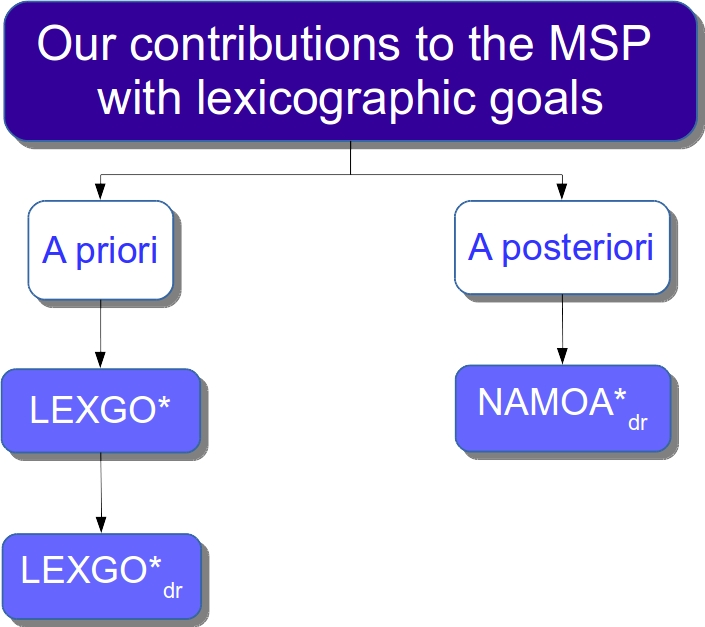
\includegraphics[scale=0.4]{figs/contributions}
	\end{figure}
\note{}
\end{frame}
%%%%%%%%%%%%%%%%%%%%%%%%%%%%%%%%%%%%%%%%%%%%%%%%%%%%%%%%%%%%%%%%%%%%%%%%%%%%%%%%%%%%%%%%%%%%%%%%%%%%%%%%%
\subsection{\texorpdfstring{\lexgo}{\lexgo}}
\begin{frame}
\frametitle{Lexicographic goal preferences}
	\begin{alertblock}{Important!}
		\vspace{1mm}
		Bellman's Principle of Optimality, \textbf{an optimal path is made up of suboptimal paths}, holds for multiobjective search problems, but \textcolor{red}{it does not hold for lexicographic goal preferences!}
		\vspace{1mm}
	\end{alertblock}
\note{Let's remark a fact, the principle of optimality does hold for MSP but it does not hold for lexicographic goals. We need to keep that in mind when we present the new discarding rules for these problems.}
\end{frame}
%%%%%%%%%%%%%%%%%%%%%%%%%%%%%%%%%%%%%%%%%%%%%%%%%%%%%%%%%%%%%%%%%%%%%%%%%%%%%%%%%%%%%%%%%%%%%%%%%%%%%%%%%
\begin{frame}
\frametitle{Lexicographic goal preferences}
	\begin{example}
		\vspace{1mm}
		Two paths $P_1$ and $P_2$ reach some node $n$ with costs $\vec g(P_1) = (\textcolor<2>{red}{8}, \textcolor<2>{red}{8}, \textcolor<3>{red}{12})$ and $\vec g(P_2) = (\textcolor<2>{red}{10}, \textcolor<2>{red}{10}, \textcolor<3>{red}{8})$, respectively. The user goals are defined as follows:
		\vspace{1mm}		
	\end{example}
	\vspace{-4mm}
	\begin{columns}[onlytextwidth, t]
	\column{0.5\linewidth}
	\vspace{4mm}
    \begin{equation*}
     \begin{array}{cll}
     	\textrm{Level 1:} & g_1 \leq 10, & w_1 = 0.5 \\
     					  & g_2 \leq 10, & w_2 = 0.5 \\ 
       	\textrm{Level 2:} & g_3 \leq 10, & w_3 = 1.
     \end{array}
   \end{equation*}	
	\column{0.5\linewidth}
    \begin{figure}
    \centering
    		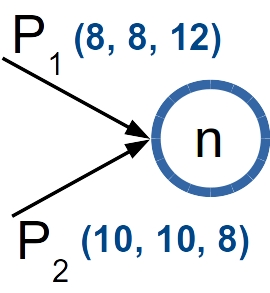
\includegraphics[scale=0.3]{figs/optimality-principle}
  	\end{figure}
	\end{columns}     
   \begin{example}
		\vspace{1mm}	
		The deviation from goals for $P_1$ and $P_2$ is $\vec d(P_1) = (\textcolor<2>{red}{0}, \textcolor<3>{red}{2})$ and $\vec d(P_2) = (\textcolor<2>{red}{0}, \textcolor<3>{red}{0})$, respectively. Thus, \textcolor{ao}{$P_2 \prec_G P_1$}.
		\vspace{1mm}	
	\end{example}
\note{}
\end{frame}
%%%%%%%%%%%%%%%%%%%%%%%%%%%%%%%%%%%%%%%%%%%%%%%%%%%%%%%%%%%%%%%%%%%%%%%%%%%%%%%%%%%%%%%%%%%%%%%%%%%%%%%%%
\begin{frame}
\frametitle{Lexicographic goal preferences}
	\begin{example}
		\vspace{1mm}	
		Let's now consider there is only one additional path $P_3$ to the destination node $t$, such as $\vec g(P_3)) = (2, 2, 2)$. \\
		Therefore, \\ 
		\begin{itemize}
			\item $\vec g(P_1 P_3)) = (\textcolor<2>{red}{10}, \textcolor<2>{red}{10}, \textcolor<3>{red}{14})$ and $\vec g(P_2 P_3)) = (\textcolor<2>{red}{12}, \textcolor<2>{red}{12}, \textcolor<3>{red}{10})$. 
			\item $\vec d(P_1 P_3) = (\textcolor<2>{red}{0},\textcolor<3>{red}{4})$ and $\vec d(P_2 P_3) = (\textcolor<2>{red}{2},\textcolor<3>{red}{0})$. 
			\item Now, \textcolor{ao}{$P_1 P_3 \prec_G P_2 P_3$}
		\end{itemize}
		\textcolor{red}{We have pruned an optimal path!}
		\vspace{1mm}	
	\end{example}
	\begin{figure}
    \centering
    		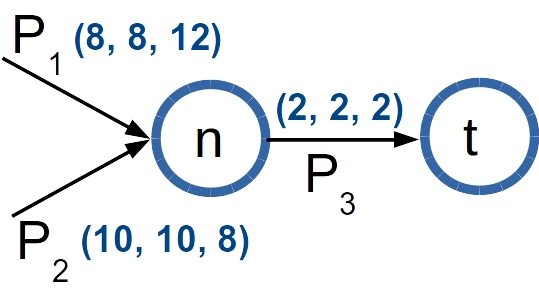
\includegraphics[scale=0.3]{figs/optimality-principle2}
  	\end{figure}
\note{}
\end{frame}
%%%%%%%%%%%%%%%%%%%%%%%%%%%%%%%%%%%%%%%%%%%%%%%%%%%%%%%%%%%%%%%%%%%%%%%%%%%%%%%%%%%%%%%%%%%%%%%%%%%%%%%%%
\begin{frame}
\frametitle{Lexicographic goal preferences}
	\begin{example}
		Let's now assume paths $P_1$ and $P_2$ have costs $\vec g(P_1)$ = (\textcolor<2>{red}{12}, \textcolor<3>{red}{8, 16}) and $\vec g(P_2)$ = (\textcolor<2>{red}{12}, \textcolor<3>{red}{12, 6}), respectively. The user goals are now \emph{different} and defined as follows:
	\end{example}
	\vspace{-6mm}
	\begin{columns}[onlytextwidth, t]
	\column{0.5\linewidth}
	\vspace{3mm}
    \begin{equation*}
     \begin{array}{cll}
     	\textrm{Level 1:} & g_1 \leq 10, & w_1 = 1 \\
     	\textrm{Level 2:} & g_2 \leq 10, & w_2 = 0.5 \\ 
       	 				  & g_3 \leq 10, & w_3 = 0.5. \\
     \end{array}
   \end{equation*}	
	\column{0.5\linewidth}
    \begin{figure}
    \centering
    		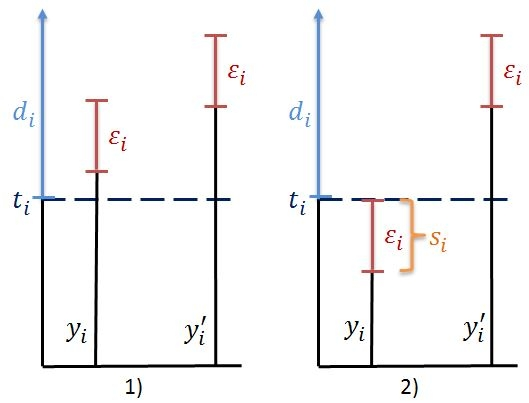
\includegraphics[scale=0.25]{figs/cross-slacks}
  	\end{figure}
	\end{columns}     
   \begin{example}
		The deviation from goals for $P_1$ and $P_2$ is now $\vec d(P_1)$ = (\textcolor<2>{red}{2}, \textcolor<3>{red}{3}) and $\vec d(P_2)$ = (\textcolor<2>{red}{2}, \textcolor<3>{red}{1}), respectively. $P_2 \prec_G P_1$, but, can $P_1$ be \textcolor{red}{safely} pruned?
	\end{example}
\note{}
\end{frame}
%%%%%%%%%%%%%%%%%%%%%%%%%%%%%%%%%%%%%%%%%%%%%%%%%%%%%%%%%%%%%%%%%%%%%%%%%%%%%%%%%%%%%%%%%%%%%%%%%%%%%%%%%
\begin{frame}
\frametitle{Discarding labels by deviation}
	Deviation-based pruning ($\prec_P$)
	\vspace{5mm}
	\begin{columns}[onlytextwidth, t]
	\column{0.35\linewidth}
	\textit{Slack variable} \\
	\vspace{1mm}	
	\Ovalbox{$s_k = \max(0, t_k - y_k)$}
	\column{0.6\linewidth}
	\textit{Cross slacks} \\
	\vspace{1mm}	
	\Ovalbox{$\delta_j(\vec{y}, \vec{y'}) = \sum_{k\in I_j} w_k \times \max(0, s'_k - s_k)$}
	\end{columns}
	\vspace{3mm}
	\begin{example}
		\vspace{1mm}
		Given $\vec g(P_1)$ = (12, \textcolor<2>{red}{8}, 16) and \ $\vec g(P_2)$ = (12, 12, \textcolor<3>{red}{6}),\\
		where $\vec d(P_1)$ = (2, \textcolor<5>{red}{3}) and \ $\vec d(P_2)$ = (2, \textcolor<5>{red}{1}):
		\begin{itemize}
			\item \textcolor<2>{red}{$s_2(P_1) = (10 - 8) \times 0.5 = \textcolor<4>{red}{1}$.} 
			\item \textcolor<3>{red}{$s_3(P_2) = (10 - 6) \times 0.5 = \textcolor<4>{red}{2}.$} 
			\item \textcolor<4>{red}{$\delta_2(P_1, P_2)= 2 - 1 = \textcolor<6>{red}{1}$,} 
		\end{itemize}
		\textcolor<5>{red}{Finally, $d_2(P_2) - d_2(P_1) = 3 - 1 = 2$} $>$ \textcolor<6>{red}{1}.
		\vspace{1mm}		
	\end{example}
\note{}
\end{frame}
%%%%%%%%%%%%%%%%%%%%%%%%%%%%%%%%%%%%%%%%%%%%%%%%%%%%%%%%%%%%%%%%%%%%%%%%%%%%%%%%%%%%%%%%%%%%%%%%%%%%%%%%%
\begin{frame}
\frametitle{Discarding labels by deviation}
Deviation-based pruning ($\prec_P$) \\
	\vspace{3mm}
     $ \vec{y} \prec_{P} \vec{y'} \ \ \Leftrightarrow \ \ $ \textcolor<2>{red}{$\forall i < j
      \ \ (d_i(\vec{y}) = d_i(\vec{y'}) \ \quad \land \quad \delta_i(\vec{y}, \vec{y'}) = 0))$} $\quad \land$ \\
     \vspace{3mm}
     \qquad \qquad \qquad \qquad \textcolor<3>{red}{$\exists j \ (d_j(\vec{y}) < d_j(\vec{y'}) \quad \land \quad \delta_j(\vec{y}, \vec {y'}) < d_j(\vec{y'}) - d_j(\vec{y})$} \\
	\vspace{5mm}
	Deviation-based filtering
	\vspace{3mm}
	\begin{equation*}
     \vec{d_B} \prec_{L} \vec{d}
    \end{equation*}
\end{frame}
%%%%%%%%%%%%%%%%%%%%%%%%%%%%%%%%%%%%%%%%%%%%%%%%%%%%%%%%%%%%%%%%%%%%%%%%%%%%%%%%%%%%%%%%%%%%%%%%%%%%%%%%%
\begin{frame}
\frametitle{\lexgo}	
	\begin{framed}
		\textcolor{ao}{In addition to the pruning and filtering rules of \namoa}, 
		\lexgo \ also uses its own rules to prune and filter paths by deviation.
	\end{framed}
\note{}
\end{frame}	
%%%%%%%%%%%%%%%%%%%%%%%%%%%%%%%%%%%%%%%%%%%%%%%%%%%%%%%%%%%%%%%%%%%%%%%%%%%%%%%%%%%%%%%%%%%%%%%%%%%%%%%%%
\begin{frame}
\frametitle{\lexgo}
	\begin{alertblock}{\lexgo \ shares \namoa \ formal properties}
		\begin{itemize}
		\vspace{2mm}
		\item The \textcolor{red}{new} deviation-based pruning and filtering rules \textcolor{red}{do not discard} goal-optimal solutions.
		\vspace{2mm}
 		\item \lexgo \ \textcolor{red}{always} returns the set of all goal-optimal solutions.
		\vspace{2mm}
 		\item \lexgo \ expands a \textcolor{red}{subset} of the labels expanded by \namoa.
 		\vspace{2mm}
		\end{itemize}
	\end{alertblock}
\note{}
\end{frame}
%%%%%%%%%%%%%%%%%%%%%%%%%%%%%%%%%%%%%%%%%%%%%%%%%%%%%%%%%%%%%%%%%%%%%%%%%%%%%%%%%%%%%%%%%%%%%%%%%%%%%%%%%
\subsection{T-discarding}
\begin{frame} 
\frametitle{T-discarding}
	\begin{block}{Limiting factor in MSP}
	\vspace{1mm}
		\textcolor{ao}{Runtime}, rather than memory, is the \textcolor{ao}{limiting factor} in multicriteria search algorithms performance, as well as in the size of problems that can be practically solved.
	\vspace{1mm}
	\end{block}
	\vspace{8mm}
	\begin{block}{Limiting factor in MSP (II)}
	\vspace{1mm}
		The \textcolor{ao}{majority} of the algorithm \textcolor{ao}{runtime} can be attributed to dominance checks against $G_{op}, G_{cl}$ and COSTS to discard dominated paths. 
	\vspace{1mm}
	\end{block}
\note{T-discarding arose due to time rather memory is nowadays the limiting factor in multicriteria search algorithms performance. This runtime can be mostly attributed to dominance checks to discard paths. In this manner, if we speed up these checks, we will speed up the algorithms.}
\end{frame}
%%%%%%%%%%%%%%%%%%%%%%%%%%%%%%%%%%%%%%%%%%%%%%%%%%%%%%%%%%%%%%%%%%%%%%%%%%%%%%%%%%%%%%%%%%%%%%%%%%%%%%%%%
\begin{frame}
\frametitle{T-discarding}
	Let's suppose a typical scenario where a new path with cost $\vec v$ reaches some node $n$. This node \textcolor{ao}{has already three closed paths} with costs $(\vec x, \vec y, \vec z)$. Let's now \textcolor{ao}{check if $\vec v$ is dominated} by any vector in $G_{cl}(n)$:
	\vspace{5mm}
	\begin{columns}%[onlytextwidth, t]
	\column{0.5\linewidth}
	\begin{example}
	\vspace{1mm}
	\begin{itemize}
		\item $\vec x \prec \vec v$ ? \ $\rightarrow$ \ $x_1 \leq v_1$, $x_2 \leq v_2$ ...
		\item $\vec y \prec \vec v$ ? \ $\rightarrow$ \ $y_1 \leq v_1$, $y_2 \leq v_2$ ...
		\item $\vec z \prec \vec v$ ? \ $\rightarrow$ \ $z_1 \leq v_1$, $z_2 \leq v_2$ ...
	\end{itemize}
	Worst-case scenario: \\ 
	\begin{itemize}
		\item 3 vector comparisons
		\item 9 scalar comparisons
	\end{itemize}
	\end{example}
	\column{0.5\linewidth}
	\begin{figure}
    	\centering
		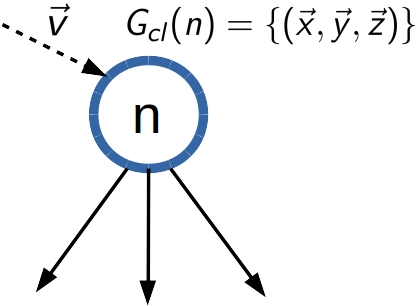
\includegraphics[scale=0.45]{figs/t-discarding}
	\end{figure}
	\end{columns}
\note{}
\end{frame}	
%%%%%%%%%%%%%%%%%%%%%%%%%%%%%%%%%%%%%%%%%%%%%%%%%%%%%%%%%%%%%%%%%%%%%%%%%%%%%%%%%%%%%%%%%%%%%%%%%%%%%%%%%
\begin{frame} 
\frametitle{T-discarding}
	\begin{block}{Definition}
		\vspace{1mm}
		T-discarding (\emph{truncated discarding}) is a dimensionality reduction technique to \textcolor{ao}{speed up dominance checks}.
		\vspace{1mm}
	\end{block}
\note{This is the definition of our proposal, called t-discarding, or truncated distarding. This proposal is based on a dimensionality reduction technique to speed up dominance checks.}
\end{frame}	
%%%%%%%%%%%%%%%%%%%%%%%%%%%%%%%%%%%%%%%%%%%%%%%%%%%%%%%%%%%%%%%%%%%%%%%%%%%%%%%%%%%%%%%%%%%%%%%%%%%%%%%%%
\begin{frame}[t]
\frametitle{T-discarding}
	\begin{block}{Assumptions}
		\vspace{1mm}
		To apply t-discarding an algorithm must have:
		\begin{itemize}
			\item Lexicographic order as label selection policy.
			\item One consistent heuristic function as lower bound. 
		\end{itemize}
		\vspace{1mm}
	\end{block}
	\only<2-3>{
	\begin{example}
	When \textcolor{ao}{lexicographic order} is used to select open paths:
	\vspace{-2mm}
	\begin{columns}[onlytextwidth, t]
	\column{0.5\linewidth}
		\begin{itemize}
			\item<2> $\rightarrow$ (3, 5, 7)
			\item<2> $\rightarrow$ (4, 6, 4)
			\item<2> $\rightarrow$ (4, 6, 7)
			\item<2> $\rightarrow$ (6, 2, 4)
		\end{itemize}
	\column{0.5\linewidth}
		\begin{itemize}
			\item<3> $\rightarrow$ (3, -, -)
			\item<3> $\rightarrow$ (4, -, -)
			\item<3> $\rightarrow$ (4, -, -)
			\item<3> $\rightarrow$ (6, -, -)
		\end{itemize}	
	\end{columns}	
	\end{example}
	}
	\only<4>{
	\vspace{5mm}	
	\begin{alertblock}{Property}
		Assuming the last selected open path had cost $\vec c = c_1, c_2, ..., c_q$, the next path selected to be open with cost $\vec{c'} = c'_1, c'_2, ..., c'_q$ \textcolor{red}{must have} $c'_1 \geq c_1$ !
	\end{alertblock}
	}
\note{Do we have some assumptions before applying this technique? Yes, two assumptions, the first one is to use a lexicographic order as label selection policy, and the second one, is to use a consistent heuristic function as lower bound.
We can depict here the main idea. This is the representation of 3 vectors x, y, and z. What happens if we ignore the first objective and we represent the three truncated vectors only according to the second and third objectives? We observe that the truncated vector x dominates the other two... 
}
\end{frame}
%%%%%%%%%%%%%%%%%%%%%%%%%%%%%%%%%%%%%%%%%%%%%%%%%%%%%%%%%%%%%%%%%%%%%%%%%%%%%%%%%%%%%%%%%%%%%%%%%%%%%%%%%
\begin{frame}
\frametitle{T-discarding}
	Let's suppose a typical scenario where a new path with cost $\vec v$ reaches some node $n$. This node \textcolor{ao}{has already three closed paths} with costs $(\vec x, \vec y, \vec z)$. Let's now \textcolor{ao}{check if $\vec v$ is dominated} by any vector in $G_{cl}(n)$:
	\vspace{5mm}
	\begin{columns}%[onlytextwidth, t]
	\column{0.5\linewidth}
	\begin{example}
	\vspace{1mm}
	\begin{itemize}
		\item $\vec x \prec \vec v$ ? \ $\rightarrow$ \ $x_1 \leq v_1$, $x_2 \leq v_2$ ...
		\item $\vec y \prec \vec v$ ? \ $\rightarrow$ \ $y_1 \leq v_1$, $y_2 \leq v_2$ ...
		\item $\vec z \prec \vec v$ ? \ $\rightarrow$ \ $z_1 \leq v_1$, $z_2 \leq v_2$ ...
	\end{itemize}
	Worst-case scenario: \\ 
	\begin{itemize}
		\item 3 vector comparisons
		\item 9 scalar comparisons
	\end{itemize}
	\end{example}
	\column{0.5\linewidth}
	\begin{figure}
    	\centering
		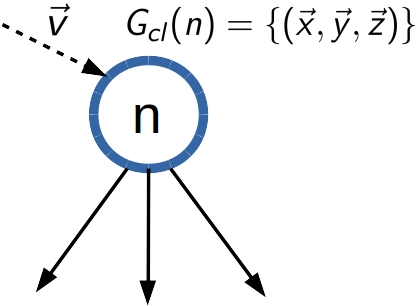
\includegraphics[scale=0.45]{figs/t-discarding}
	\end{figure}
	\end{columns}
\note{}
\end{frame}	
%%%%%%%%%%%%%%%%%%%%%%%%%%%%%%%%%%%%%%%%%%%%%%%%%%%%%%%%%%%%%%%%%%%%%%%%%%%%%%%%%%%%%%%%%%%%%%%%%%%%%%%%%
\begin{frame}
\frametitle{T-discarding}
	\begin{figure}
    	\centering
		\includegraphics<1>[scale=0.4]{figs/t-discarding1}
		\includegraphics<2>[scale=0.4]{figs/t-discarding2}
		\includegraphics<3>[scale=0.4]{figs/t-discarding3}
	\end{figure}
\note{}
\end{frame}
%%%%%%%%%%%%%%%%%%%%%%%%%%%%%%%%%%%%%%%%%%%%%%%%%%%%%%%%%%%%%%%%%%%%%%%%%%%%%%%%%%%%%%%%%%%%%%%%%%%%%%%%%
\begin{frame}
\frametitle{T-discarding}
	Let's suppose a typical scenario where a new path with cost $\vec v$ reaches some node $n$. This node \textcolor{ao}{has already three closed paths} with costs $(\vec x, \vec y, \vec z)$. Let's now \textcolor{ao}{check if $\vec v$ is dominated} by any vector in $G_{cl}(n)$:
	\vspace{5mm}
	\begin{columns}%[onlytextwidth, t]
	\column{0.5\linewidth}
	\begin{example}
	\vspace{1mm}
	\begin{itemize}
		\item $\vec x \prec \vec v$ ? \ $\rightarrow$ \ $x_1 \leq v_1$, $x_2 \leq v_2$ ...
		\item $\vec y \prec \vec v$ ? \ $\rightarrow$ \ $y_1 \leq v_1$, $y_2 \leq v_2$ ...
		\item $\vec z \prec \vec v$ ? \ $\rightarrow$ \ $z_1 \leq v_1$, $z_2 \leq v_2$ ...
	\end{itemize}
	Worst-case scenario: \\ 
	\begin{itemize}
		\item 3 vector comparisons
		\item 9 scalar comparisons
	\end{itemize}
	\end{example}
	\column{0.5\linewidth}
	\begin{figure}
    	\centering
		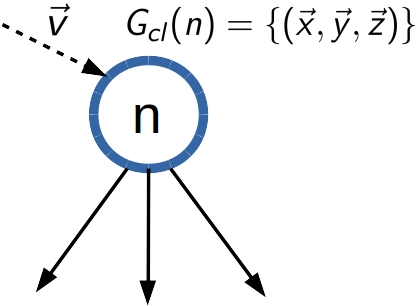
\includegraphics[scale=0.45]{figs/t-discarding}
	\end{figure}
	\end{columns}
\note{}
\end{frame}	
%%%%%%%%%%%%%%%%%%%%%%%%%%%%%%%%%%%%%%%%%%%%%%%%%%%%%%%%%%%%%%%%%%%%%%%%%%%%%%%%%%%%%%%%%%%%%%%%%%%%%%%%%
\begin{frame}
\frametitle{T-discarding}
	Is a vector \textcolor{ao}{$\vec v$ dominated} by any vector in the previous set $(\vec x, \vec y, \vec z)$? 
	\vspace{8mm}
	\begin{block}{Standard discarding}
	\vspace{1mm}
	$\vec v$ \textcolor{ao}{must be compared to} $(\vec x, \vec y, \vec z)$ to check if it is dominated.
	\vspace{1mm} 
	\end{block}
	\vspace{3mm}
	\begin{block}{T-discarding}
	\vspace{1mm}
	 The truncated vector $t(\vec v)$ \textcolor{ao}{must be compared only to} $t(\vec x)$ to check if it is dominated. 
	 \vspace{1mm}
	\end{block}			
\note{}
\end{frame}
%%%%%%%%%%%%%%%%%%%%%%%%%%%%%%%%%%%%%%%%%%%%%%%%%%%%%%%%%%%%%%%%%%%%%%%%%%%%%%%%%%%%%%%%%%%%%%%%%%%%%%%%%
\begin{frame}
\frametitle{T-discarding}
\begin{block}{Benefits of t-discarding}
	\vspace{1mm}
		\begin{itemize}
			\item Dominance checks can be done with vectors \textcolor{ao}{reduced in one dimension}.
			\vspace{1mm}
			\item \textcolor{ao}{The size of sets} $T(G_{cl}(n))$ and $T(COSTS)$ \textcolor{ao}{is also reduced}.
		\end{itemize}
	\vspace{1mm}
	\end{block}
	\vspace{2mm}
	\begin{alertblock}{Important!}
		\vspace{1mm}
		T-discarding only implies checking dominance against different sets:
		\begin{itemize}
			\item \textcolor{red}{Very simple implementation.}
			\vspace{1mm}
			\item Any label discarded by standard pruning \textcolor{red}{$\Longleftrightarrow$} is discarded by t-discarding.
			\vspace{1mm}
			\item \textcolor{red}{Does not affect any formal property} of the algorithm.
		\end{itemize}			
	\end{alertblock}
\note{}
\end{frame}
%%%%%%%%%%%%%%%%%%%%%%%%%%%%%%%%%%%%%%%%%%%%%%%%%%%%%%%%%%%%%%%%%%%%%%%%%%%%%%%%%%%%%%%%%%%%%%%%%%%%%%%%%
\subsection{\texorpdfstring{\namoadr}{\namoadr}}
\begin{frame} 
\frametitle{\namoadr}
	The applicability of t-discarding to \namoa \ is \textcolor{ao}{full} and straightforward:
	\vspace{4mm}
	\begin{framed}
		Cl-pruning and filtering are now performed against: 
    		\vspace{3mm}
		\begin{itemize}
			\item $T(G_{cl}(n))$
			\vspace{3mm}
			\item T(COSTS)
		\end{itemize} 	 
	\end{framed} 
\note{}
\end{frame}
%%%%%%%%%%%%%%%%%%%%%%%%%%%%%%%%%%%%%%%%%%%%%%%%%%%%%%%%%%%%%%%%%%%%%%%%%%%%%%%%%%%%%%%%%%%%%%%%%%%%%%%%%
\subsection{\texorpdfstring{\lexgodr}{\lexgodr}}
\begin{frame} 
\frametitle{\lexgodr}
	The applicability of t-discarding to \lexgo \ is \textcolor{red}{partial}:
	\vspace{4mm}
	\begin{framed}
		Cl-pruning and filtering are now performed against: 
    		\vspace{3mm}
		\begin{itemize}
			\item $T(G_{cl}(n))$
			\vspace{3mm}
			\item T(COSTS)
		\end{itemize} 
		\vspace{3mm}	
		but \textcolor{red}{only when $\vec d = 0$}. 
	\end{framed} 
\note{}
\end{frame}
%%%%%%%%%%%%%%%%%%%%%%%%%%%%%%%%%%%%%%%%%%%%%%%%%%%%%%%%%%%%%%%%%%%%%%%%%%%%%%%%%%%%%%%%%%%%%%%%%%%%%%%%%
\begin{frame}
\frametitle{Summary}
	\begin{table}
	\centering
	\scalebox{1}{
	\begin{tabular}{|lllll|}
	\hline \noalign{\smallskip}
	& \namoa & \lexgo & \namoadr & \lexgodr \\
	\noalign{\smallskip} \hline \noalign{\smallskip}
	Op-pruning & $G_{op}(n)$ & $G_{op}(n)$ & $G_{op}(n)$ & $G_{op}(n)$ \\
	\noalign{\smallskip} \hline \noalign{\smallskip}
	Cl-pruning & $G_{cl}(n)$ & $G_{cl}(n)$ & $T(G_{cl}(n))$ & $T(G_{cl}(n))$* \\
	\noalign{\smallskip} \hline \noalign{\smallskip}
	Filtering & COSTS & COSTS & T(COSTS) & T(COSTS)* \\
	\noalign{\smallskip} \hline \noalign{\smallskip}
	\end{tabular}
	}
	\end{table}
\note{}
\end{frame}


% Formal and empirical analyses
% -----------------------------------------------------------------------------
%---------------------------------------------------------------------
%
%                          analyses.tex
%
%---------------------------------------------------------------------
%
% analyses.tex
% Copyright 2015 Dr. Francisco J. Pulido
%
% This presentation belongs to the PhD titled "New Techniques and Algorithms for Multiobjective and Lexicographic Goal-Based Shortest Path Problems", distributed under the Creative Commons Licence Attribution-NonCommercial-NoDerivs 3.0, available in http://creativecommons.org/licenses/by-nc-nd/3.0/. The complete PhD dissertation is freely accessible from http://www.lcc.uma.es/~francis/

\section{Empirical analyses}
%%%%%%%%%%%%%%%%%%%%%%%%%%%%%%%%%%%%%%%%%%%%%%%%%%%%%%%%%%%%%%%%%%%%%%%%%%%%%%%%%%%%%%%%%%%%%%%%%%%%%%%%%
\begin{frame} 
\frametitle{Empirical analyses}
\Large
	\begin{itemize}
		\item Are these new algorithms \textcolor{ao}{effective}?
		\vspace{3mm}
		\item Will \lexgo \ become faster when goals get \textcolor{ao}{more restrictive}?
		\vspace{3mm}
		\item Have we achieved \textcolor{ao}{improvements over \namoa}? \\ 
		To what extent? Why?
	\end{itemize}
\end{frame}
%%%%%%%%%%%%%%%%%%%%%%%%%%%%%%%%%%%%%%%%%%%%%%%%%%%%%%%%%%%%%%%%%%%%%%%%%%%%%%%%%%%%%%%%%%%%%%%%%%%%%%%%%
\begin{frame} 
\frametitle{Empirical analyses}
\begin{columns}[onlytextwidth, t]
\column{0.5\linewidth}
	\textbf{Random grids}
	\begin{itemize}
		\item 100 $\times$ 100
		\item \textcolor{ao}{Solution depth from 20 to 100}
		\item Random costs in range [1,10]
	\end{itemize}
	\vspace{2mm}
	\begin{figure}
    	\centering
		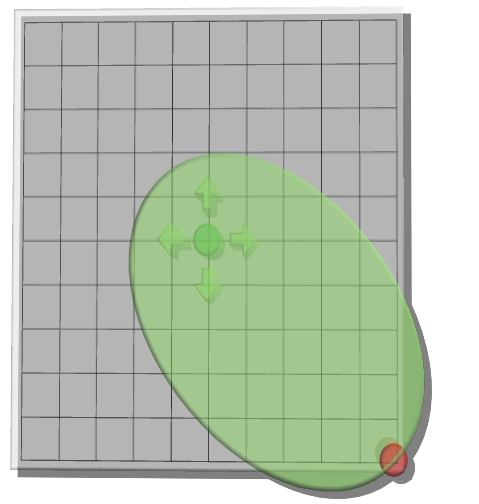
\includegraphics[scale=0.18]{figs/grids}
	\end{figure}
\column{0.5\linewidth}
	\textbf{Realistic Road maps}
	\begin{itemize}
		\item 20 random problems over \\ New York City \& Vermont State from 9th DIMACS Challenge
		\item \textcolor{ao}{Three} integer costs
		\begin{itemize}
			\item Distance 
			\item Travel time
			\item Economic cost
		\end{itemize}
	\end{itemize}
	\vspace{-5mm}
	\begin{figure}
    	\centering
		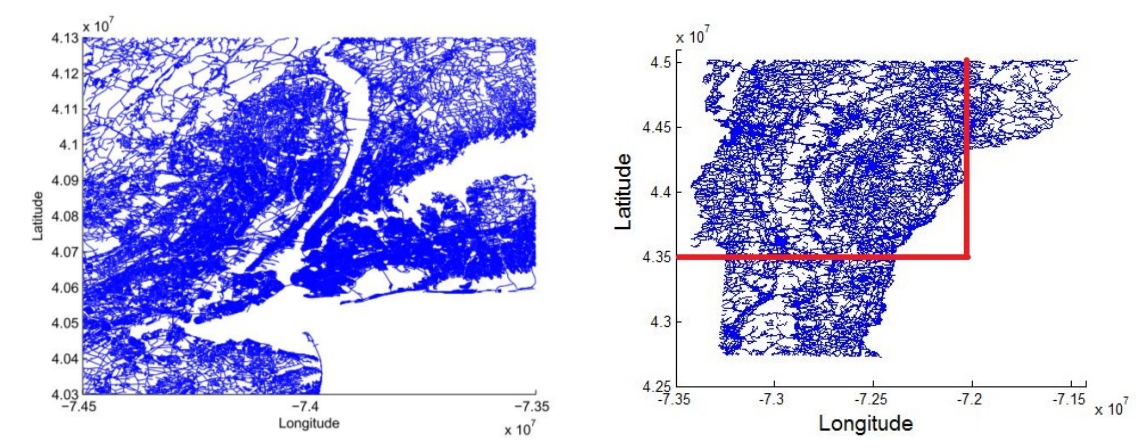
\includegraphics[scale=0.2]{figs/road_maps}
  	\end{figure}
\end{columns} 
\note{This research work employed two different benchmarks, random grids and realistic road maps.  The first experiments were performed on 100 times 100 grids with the start node located in the center of the grid and the target node at different solutions depths from 20 to 100 to the bottom right corner. Horizontal and vertical movements are possible in the grid, with arcs costs randomly generated from one to ten for each of the $q$ criteria. 

We also tested the algorithms in two maps from the 9th DIMACS Shortest Path Challenge, with three metrics, distance and travel time, and the economic cost, calculated as a function of fuel consumption, road types and tolls.}
\end{frame}
%%%%%%%%%%%%%%%%%%%%%%%%%%%%%%%%%%%%%%%%%%%%%%%%%%%%%%%%%%%%%%%%%%%%%%%%%%%%%%%%%%%%%%%%%%%%%%%%%%%%%%%%%
\subsection{Empirical analysis on grids}
\begin{frame}<beamer>[noframenumbering]
\frametitle{Empirical analyses}
	\begin{center}
		\LARGE{\textcolor{ao}{A priori}}
	\end{center}
	\begin{table}
	\centering
	\scalebox{1.5}{
	\begin{tabular}{|lll|}
	\hline \noalign{\smallskip}
	\lexgo & vs & \namoa\\
	\noalign{\smallskip} \hline \noalign{\smallskip}
	\end{tabular}
	}
	\end{table}
\note{}
\end{frame}
 %%%%%%%%%%%%%%%%%%%%%%%%%%%%%%%%%%%%%%%%%%%%%%%%%%%%%%%%%%%%%%%%%%%%%%%%%%%%%%%%%%%%%%%%%%%%%%%%%%%%%%%%%
\begin{frame} 
\frametitle{\lexgo \ vs \namoa}
	\begin{figure}
    	\centering
		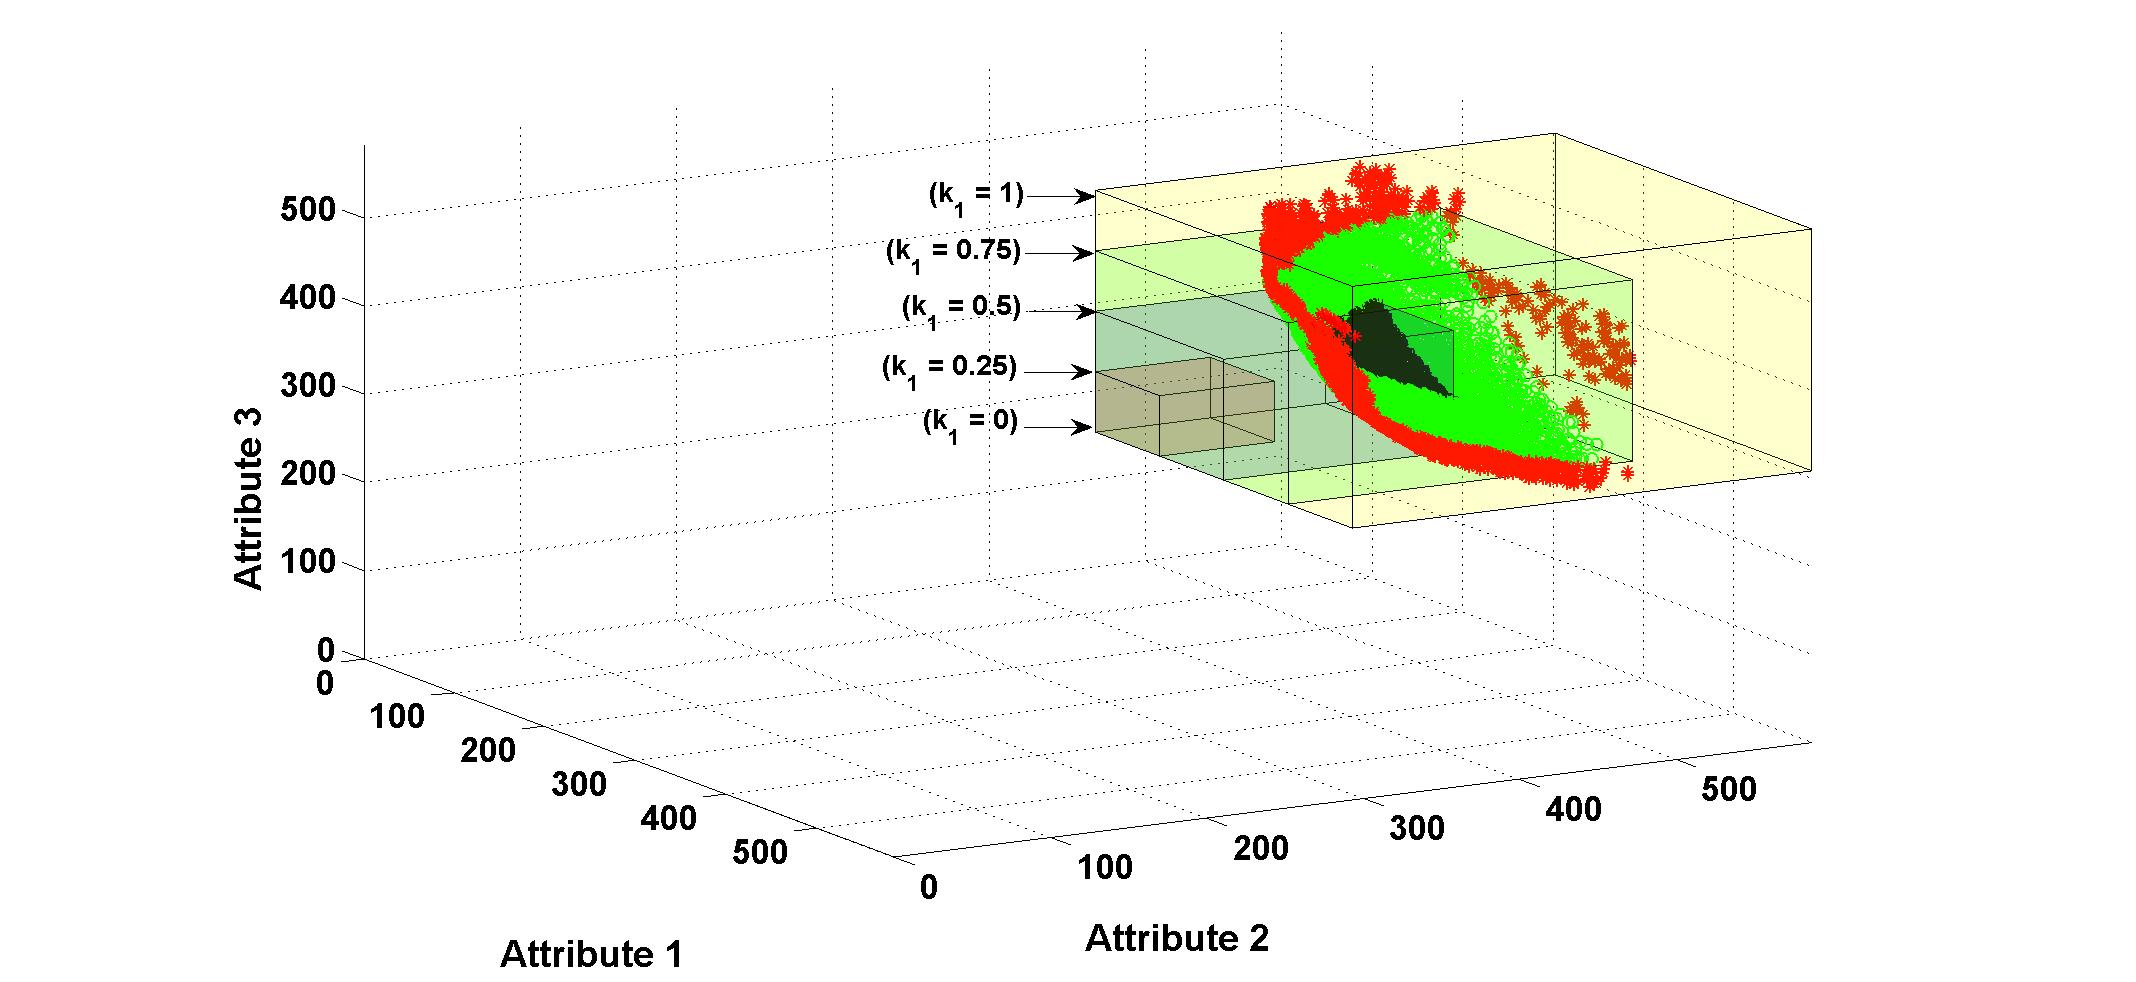
\includegraphics[scale=0.175]{figs/lexgo3d}
	\caption{3D Pareto frontier according to goal satisfiability.}
	\end{figure}
\note{In this figure we see the three dimensional Pareto frontier obtained by \namoa \ for a grid problem. Each of these cubes represent the goals imposed to \lexgo \ in Class I experiments, from the ideal point, located on $k_1$ equals to zero, to the yellow cube that corresponds to goals situated in the nadir point. We can observe that in 0.5 a good percentage of the Pareto frontier would be returned by \lexgo, and in 0.75 the majority of the non-dominated solutions}
\end{frame}
%%%%%%%%%%%%%%%%%%%%%%%%%%%%%%%%%%%%%%%%%%%%%%%%%%%%%%%%%%%%%%%%%%%%%%%%%%%%%%%%%%%%%%%%%%%%%%%%%%%%%%%%%
\begin{frame} 
\frametitle{\lexgo \ vs \namoa}
	\begin{figure}
    	\centering
		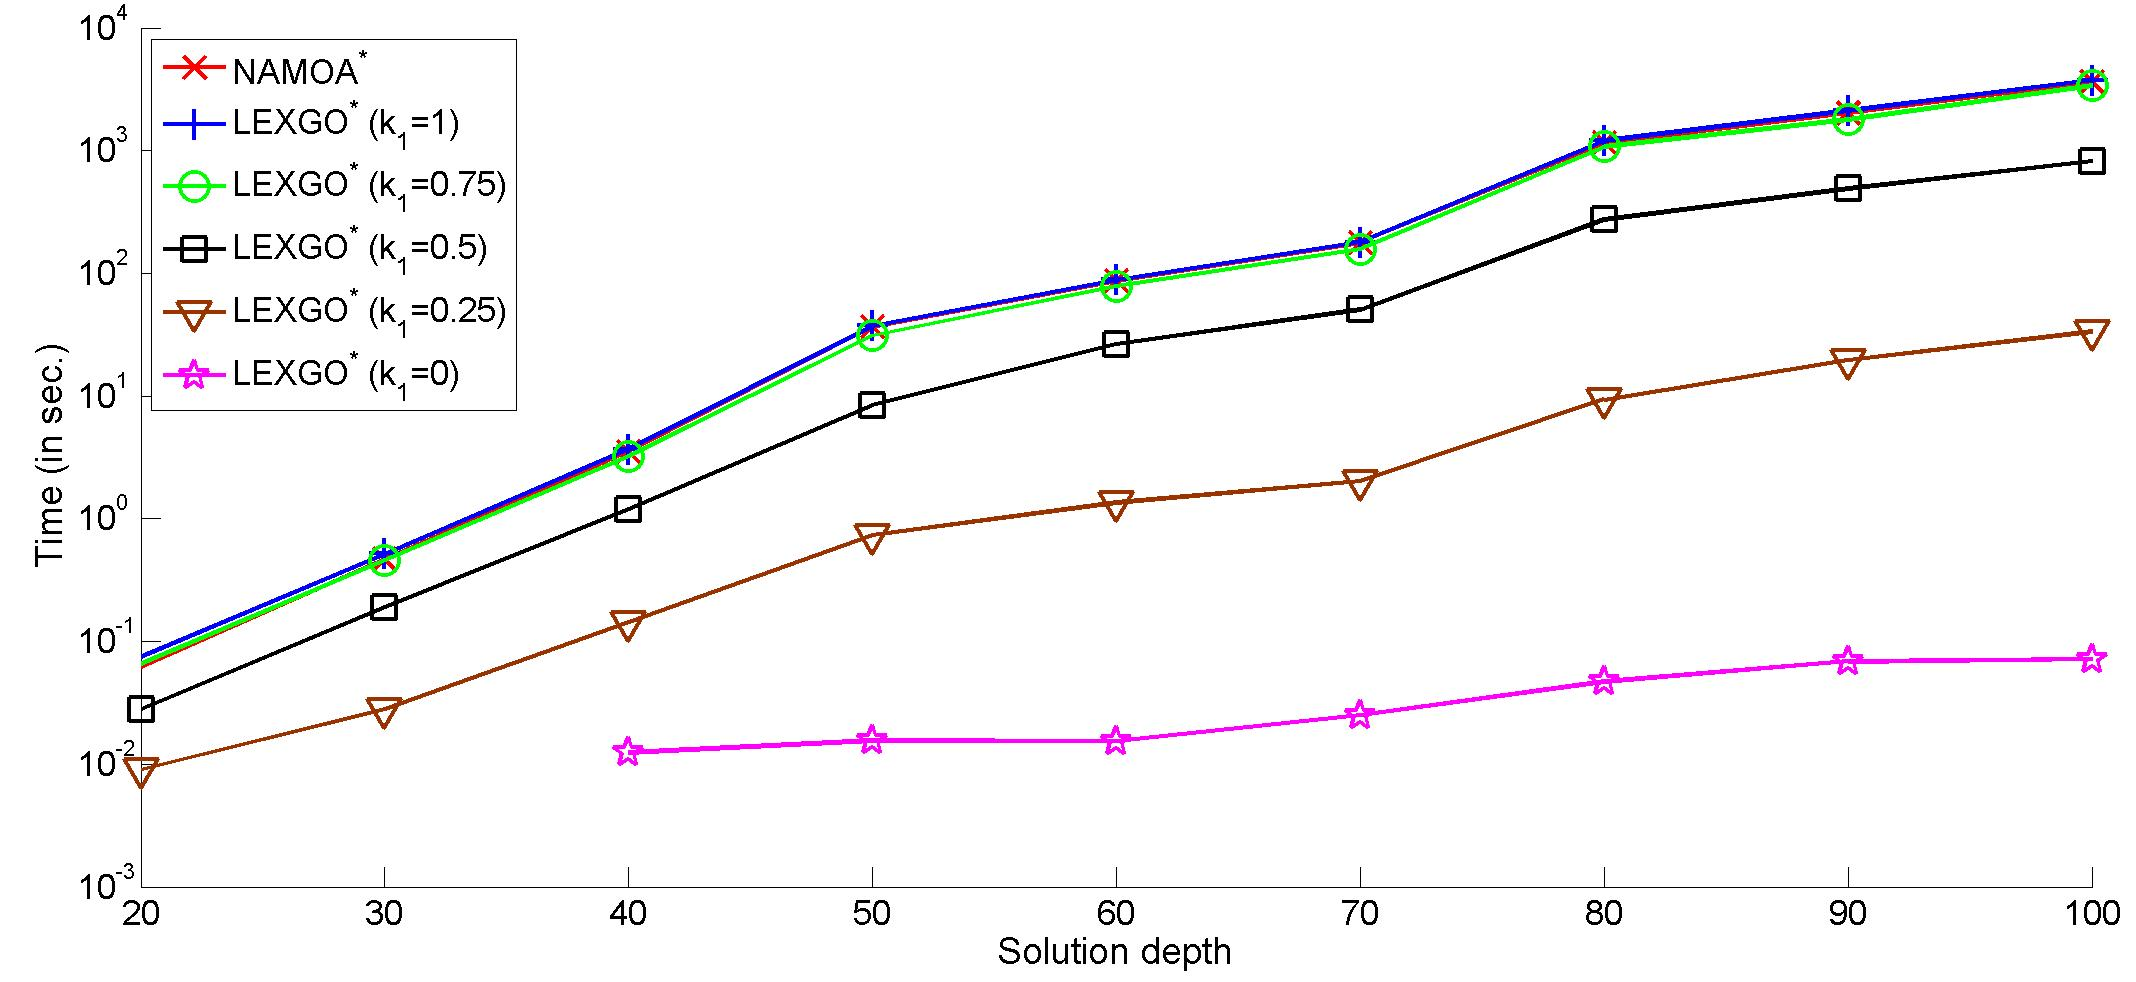
\includegraphics[scale=0.16]{figs/lexgo-exe-time}
		\caption{Runtimes of \namoa \ and \lexgo \ in seconds (logarithmic scale).}
	\end{figure}
\note{}
\end{frame}
%%%%%%%%%%%%%%%%%%%%%%%%%%%%%%%%%%%%%%%%%%%%%%%%%%%%%%%%%%%%%%%%%%%%%%%%%%%%%%%%%%%%%%%%%%%%%%%%%%%%%%%%%
\begin{frame}[t]
\frametitle{\lexgo \ vs \namoa}
	\vspace{5mm}
	\begin{center}
		\begin{table}
		\caption{%
    		Runtimes for $d = 100$ experiments.
     	}%
     	\vspace{2mm}
     		\scalebox{1.2}{
			\begin{tabular}{rrrrrrr}
			\hline \noalign{\smallskip}
			& \multicolumn{5}{c}{\lexgolex} \\
			\noalign{\smallskip} \cline{2-6} \noalign{\smallskip}
			\namoalex & 1 & 0.75 & 0.5 & 0.25 & 0 & \multicolumn{1}{c}{$k_1$} \\
			\noalign{\smallskip} 
			Runtime (s) & \% & \% & \% & \% & \% \\
			\cline{1-6}  \noalign{\smallskip} 
			3,662.9 & 102.7 & \textcolor{ao}{92.3} & \textcolor{ao}{22.3} & \textcolor{ao}{0.9} & \textcolor{ao}{0.001} \\
			\hline
			\end{tabular} 
			}
		\end{table}
	\end{center}
\note{Let's see now the runtime requirements. We also observe here the effectiveness of \lexgo, 5 orders of magnitude faster for k1 equals to 0, two orders of magnitude for k1 in 0.25, 5 times faster for 0.5, slightly faster for 0.75 and with a little overhead when \lexgo \ returns the whole Pareto frontier.
In Class experiments we observe a similar behaviour, \lexgo \ is somewhat around forty to fifty times faster than \namoa \ in these cases (0.75-0.1875, 0.5,0.125)}
\end{frame}
%%%%%%%%%%%%%%%%%%%%%%%%%%%%%%%%%%%%%%%%%%%%%%%%%%%%%%%%%%%%%%%%%%%%%%%%%%%%%%%%%%%%%%%%%%%%%%%%%%%%%%%%%
\begin{frame}<beamer>[noframenumbering]
\frametitle{Empirical analyses}
	\begin{center}
		\LARGE{\textcolor{ao}{A priori}}
	\end{center}
	\begin{table}
	\centering
	\scalebox{1.5}{
	\begin{tabular}{|lll|}
	\hline \noalign{\smallskip}
	\lexgo & vs & \namoa\\
	\noalign{\smallskip} \hline \noalign{\smallskip}
	\lexgodr & vs & \lexgo\\
	\noalign{\smallskip} \hline \noalign{\smallskip}
	\end{tabular}
	}
	\end{table}
\note{}
\end{frame}
%%%%%%%%%%%%%%%%%%%%%%%%%%%%%%%%%%%%%%%%%%%%%%%%%%%%%%%%%%%%%%%%%%%%%%%%%%%%%%%%%%%%%%%%%%%%%%%%%%%%%%%%%
\begin{frame} 
\frametitle{\lexgodr \ vs \lexgo}
	\begin{figure}
    	\centering
		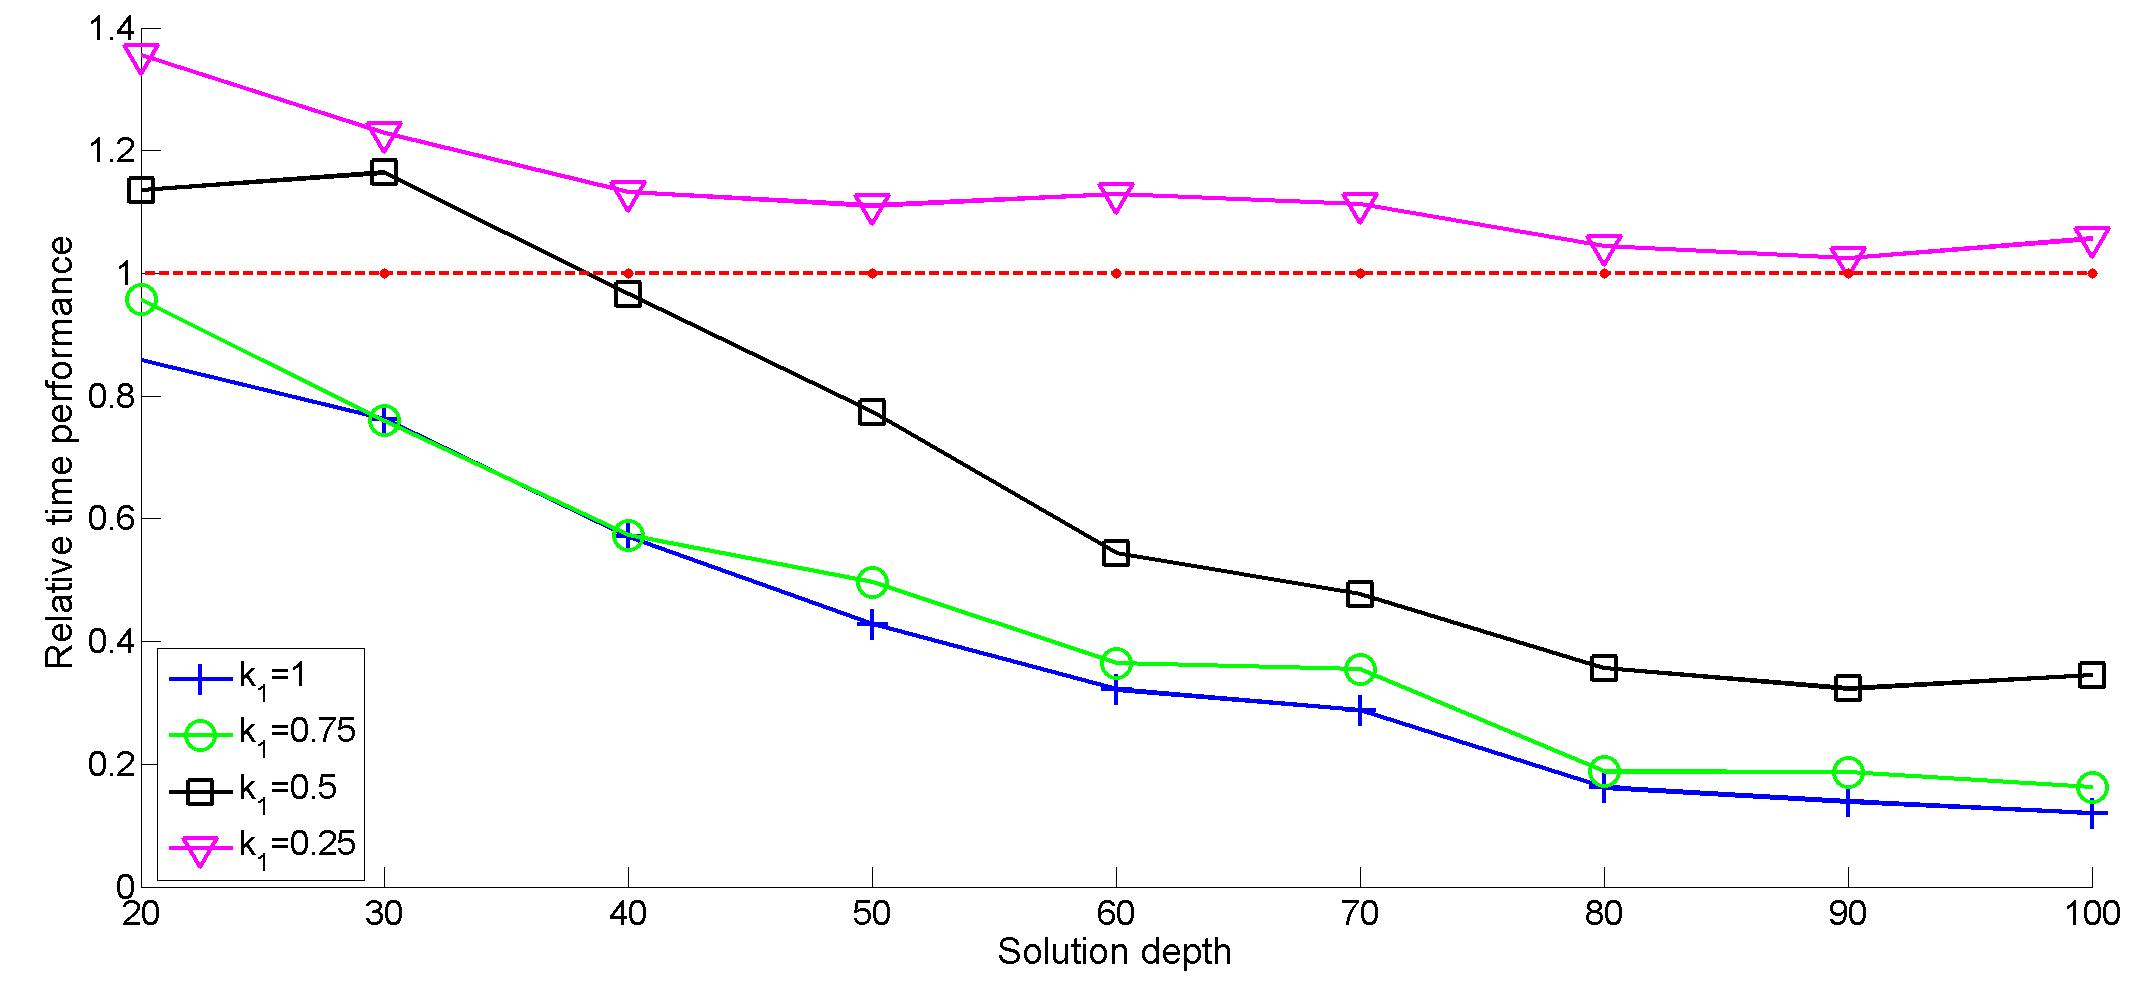
\includegraphics[scale=0.16]{figs/lexgodr-exe-time}
		\caption{Relative runtime performance of \lexgodr \ over \lexgo.}
	\end{figure}
\note{}
\end{frame}
%%%%%%%%%%%%%%%%%%%%%%%%%%%%%%%%%%%%%%%%%%%%%%%%%%%%%%%%%%%%%%%%%%%%%%%%%%%%%%%%%%%%%%%%%%%%%%%%%%%%%%%%%
\begin{frame} 
\frametitle{\lexgodr \ vs \lexgo}
	\begin{table}
	\caption{Runtimes in seconds for $d = 100$ experiments.}
	\vspace{2mm}
	\centering
	\scalebox{1.2}{
	\begin{tabular}{rrrr}
	%\hline \noalign{\smallskip}
	\cline{2-4} \noalign{\smallskip}
	$k_1$ & \lexgolex & \lexgodr & Speedup\\
	\noalign{\smallskip} \hline
	1 & 3,763.78 & 254.40 & \textcolor{ao}{14.81} \\
	0.75 & 3,381.33 & 300.86 & \textcolor{ao}{11.27} \\
	0.5 & 819.28 & 282.49 & \textcolor{ao}{2.90} \\
	0.25 & 33.47 & 35.37 & 0.94 \\
	0 & 0.07 & 0.10 & 0.7\\
	\hline
	\end{tabular}
	}
	\end{table}
\note{Is t-discarding as effective in \lexgo \ as it was in \namoa? To some extent, we see speed ups of 2 to 8 when goals can be satisfied, and obviously nothing we goals can not be satisfied, since t-discarding is not applied then.}
\end{frame}
%%%%%%%%%%%%%%%%%%%%%%%%%%%%%%%%%%%%%%%%%%%%%%%%%%%%%%%%%%%%%%%%%%%%%%%%%%%%%%%%%%%%%%%%%%%%%%%%%%%%%%%%%
\begin{frame}<beamer>[noframenumbering]
\frametitle{Empirical analyses}
	\begin{center}
		\LARGE{\textcolor{ao}{A posteriori}}
	\end{center}
	\begin{table}
	\centering
	\scalebox{1.5}{
	\begin{tabular}{|lll|}
	\hline \noalign{\smallskip}
	\namoadr & vs & \namoa\\
	\noalign{\smallskip} \hline \noalign{\smallskip}
	\end{tabular}
	}
	\end{table}
\note{}
\end{frame}
 %%%%%%%%%%%%%%%%%%%%%%%%%%%%%%%%%%%%%%%%%%%%%%%%%%%%%%%%%%%%%%%%%%%%%%%%%%%%%%%%%%%%%%%%%%%%%%%%%%%%%%%%%
\begin{frame} 
\frametitle{\namoadr \ vs \namoa}
	\begin{figure}
    	\centering
		\includegraphics<1>[scale=0.075]{figs/namoas-exe}
		\caption{Runtimes for \namoalex, \namoalin, and \namoadr \ with $q = \{3, 4, 5\}$}		 
	\end{figure}
\note{We see these improvements here. For three, four or five objectives, the runtimes are greatly reduced and the improvement even grows with problem difficulty. In particular, for three objectives we see here a comparison between the new \namoa \ and both versions of standard \namoa \ with lexicographic and linear selection orders. I'd like to remark that like in other studies, \namoalin \ is somewhat twice as fast as \namoalex, but both are meaningfully slower than \namoadr.}
\end{frame}
%%%%%%%%%%%%%%%%%%%%%%%%%%%%%%%%%%%%%%%%%%%%%%%%%%%%%%%%%%%%%%%%%%%%%%%%%%%%%%%%%%%%%%%%%%%%%%%%%%%%%%%%%
\begin{frame}<beamer>[noframenumbering]
\frametitle{Empirical analyses}
	\begin{center}
		\LARGE{\textcolor{ao}{A posteriori \ vs \ A priori}}
	\end{center}
	\begin{table}
	\centering
	\scalebox{1.5}{
	\begin{tabular}{|lll|}
	\hline \noalign{\smallskip}
	\namoadr & vs & \lexgodr\\
	\noalign{\smallskip} \hline
	\end{tabular}
	}
	\end{table}
\note{}
\end{frame}
%%%%%%%%%%%%%%%%%%%%%%%%%%%%%%%%%%%%%%%%%%%%%%%%%%%%%%%%%%%%%%%%%%%%%%%%%%%%%%%%%%%%%%%%%%%%%%%%%%%%%%%%%
\begin{frame} 
\frametitle{\lexgodr \ vs \namoadr}
	\begin{table}
	\caption{Runtimes of \textcolor{ao}{\lexgodr} \ and \textcolor{red}{\namoadr}.}
	\vspace{2mm}
	\centering
	\scalebox{.9}{
	\begin{tabular}{rrrrrr}
	\hline \noalign{\smallskip}
	 & \multicolumn{5}{c}{\lexgodr} \\
	\noalign{\smallskip} \cline{2-6} \noalign{\smallskip}
	\namoadr & $(k_1=1)$ & $(k_1=0.75)$ & $(k_1=0.5)$ & $(k_1=0.25)$ & $(k_1=0)$ \\
	\noalign{\smallskip} 
	Runtime (s) \\
	\hline  \noalign{\smallskip} 
	100\% & \textcolor{red}{129.7\%} & \textcolor{red}{153.4\%} & \textcolor{red}{144\%} & \textcolor{ao}{18\%} & \textcolor{ao}{0.04\%} \\
	\hline
	\end{tabular}
	}
	\end{table} 
\note{What about the final comparison between the two best alternatives? \namoadr \ is preferable whenever a big amount of non-dominated paths satisfy the goals, and \lexgodr \ when a small number satisfy the goals or they can not be satisfied at all.}
\end{frame}
%%%%%%%%%%%%%%%%%%%%%%%%%%%%%%%%%%%%%%%%%%%%%%%%%%%%%%%%%%%%%%%%%%%%%%%%%%%%%%%%%%%%%%%%%%%%%%%%%%%%%%%%%
\subsection{Empirical analysis on road maps}
\begin{frame}<beamer>[noframenumbering]
\frametitle{Empirical analyses}
	\begin{center}
		\LARGE{\textcolor{ao}{A priori}}
	\end{center}
	\begin{table}
	\centering
	\scalebox{1.5}{
	\begin{tabular}{|lll|}
	\hline \noalign{\smallskip}
	\lexgo & vs & \namoa\\
	\noalign{\smallskip} \hline \noalign{\smallskip}
	\end{tabular}
	}
	\end{table}
\note{}
\end{frame}
 %%%%%%%%%%%%%%%%%%%%%%%%%%%%%%%%%%%%%%%%%%%%%%%%%%%%%%%%%%%%%%%%%%%%%%%%%%%%%%%%%%%%%%%%%%%%%%%%%%%%%%%%%
\begin{frame} 
\frametitle{\lexgo \ vs \namoa}
	\begin{table}
		\caption{Experiments for Vermont State map.}
		\scalebox{1.1}{
		\begin{tabular}{rrrrrrr}
		\hline \noalign{\smallskip}
		 & \multicolumn{5}{c}{\lexgolex} \\
		\noalign{\smallskip} \cline{2-6} \noalign{\smallskip}
		\namoalex & 1 & 0.75 & 0.5 & 0.25 & 0 & \multicolumn{1}{c}{$k_1$}\\
		\noalign{\smallskip} 
		Avg. runtime (s) & \% & \% & \% & \% & \% & \\
		\cline{1-6} \noalign{\smallskip} 
		5,048.47 & 100.39 & \textcolor{ao}{74.67} & \textcolor{ao}{29.06} & \textcolor{ao}{3.51} & \textcolor{ao}{0.01} \\
		\hline
		\end{tabular}
		}
	\end{table}
\note{The runtime requirements are also equivalent to the relative performance shown in grids, with greater advantage of \lexgo \ when goals are more restrictive and less non-dominated paths satisfy the goals.}
\end{frame}
%%%%%%%%%%%%%%%%%%%%%%%%%%%%%%%%%%%%%%%%%%%%%%%%%%%%%%%%%%%%%%%%%%%%%%%%%%%%%%%%%%%%%%%%%%%%%%%%%%%%%%%%%
\begin{frame}<beamer>[noframenumbering]
\frametitle{Empirical analyses}
	\begin{center}
		\LARGE{\textcolor{ao}{A priori}}
	\end{center}
	\begin{table}
	\centering
	\scalebox{1.5}{
	\begin{tabular}{|lll|}
	\hline \noalign{\smallskip}
	\lexgo & vs & \namoa\\
	\noalign{\smallskip} \hline \noalign{\smallskip}
	\lexgodr & vs & \lexgo\\
	\noalign{\smallskip} \hline \noalign{\smallskip}
	\end{tabular}
	}
	\end{table}
\note{}
\end{frame}
%%%%%%%%%%%%%%%%%%%%%%%%%%%%%%%%%%%%%%%%%%%%%%%%%%%%%%%%%%%%%%%%%%%%%%%%%%%%%%%%%%%%%%%%%%%%%%%%%%%%%%%%%
\begin{frame} 
\frametitle{\lexgodr \ vs \lexgo}
	\begin{table}
	\caption{Runtimes in seconds for Vermont State map.}
	\vspace{2mm}
	\centering
	\begin{tabular}{rrrrrrrr}
	\hline \noalign{\smallskip}
 	& 1 & 0.75 & 0.5 & 0.25 & 0 & \multicolumn{1}{c}{$k_1$}\\
	\noalign{\smallskip} 
	\cline{2-6} \noalign{\smallskip} 
	\lexgolex & 5,068.00 & 3,769.51 & 1,467.00 & 177.33 & 0.03 \\
	%\lexgolin & 4,716.90 & 3,497.26 & 1,287.37 & 205.39 & 0.03 \\
	\textcolor{red}{\lexgodr} & \textcolor{ao}{94.90} &	\textcolor{ao}{83.59} & \textcolor{ao}{57.38} & \textcolor{ao}{157.02} & \textcolor{ao}{0.03} \\
	\hline
	\end{tabular}
	\end{table}
\note{The same impressive improvements can be seen when we apply t-discarding to \lexgo \ and goals can be satisfied, with 0.5, 0.75 and 1.}
\end{frame}
%%%%%%%%%%%%%%%%%%%%%%%%%%%%%%%%%%%%%%%%%%%%%%%%%%%%%%%%%%%%%%%%%%%%%%%%%%%%%%%%%%%%%%%%%%%%%%%%%%%%%%%%%
\begin{frame}<beamer>[noframenumbering]
\frametitle{Empirical analyses}
	\begin{center}
		\LARGE{\textcolor{ao}{A posteriori}}
	\end{center}
	\begin{table}
	\centering
	\scalebox{1.5}{
	\begin{tabular}{|lll|}
	\hline \noalign{\smallskip}
	\namoadr & vs & \namoa\\
	\noalign{\smallskip} \hline \noalign{\smallskip}
	\end{tabular}
	}
	\end{table}
\note{}
\end{frame}
%%%%%%%%%%%%%%%%%%%%%%%%%%%%%%%%%%%%%%%%%%%%%%%%%%%%%%%%%%%%%%%%%%%%%%%%%%%%%%%%%%%%%%%%%%%%%%%%%%%%%%%%%
\begin{frame} 
\frametitle{\namoadr \ vs \namoa}
	\begin{figure}
    	\centering
		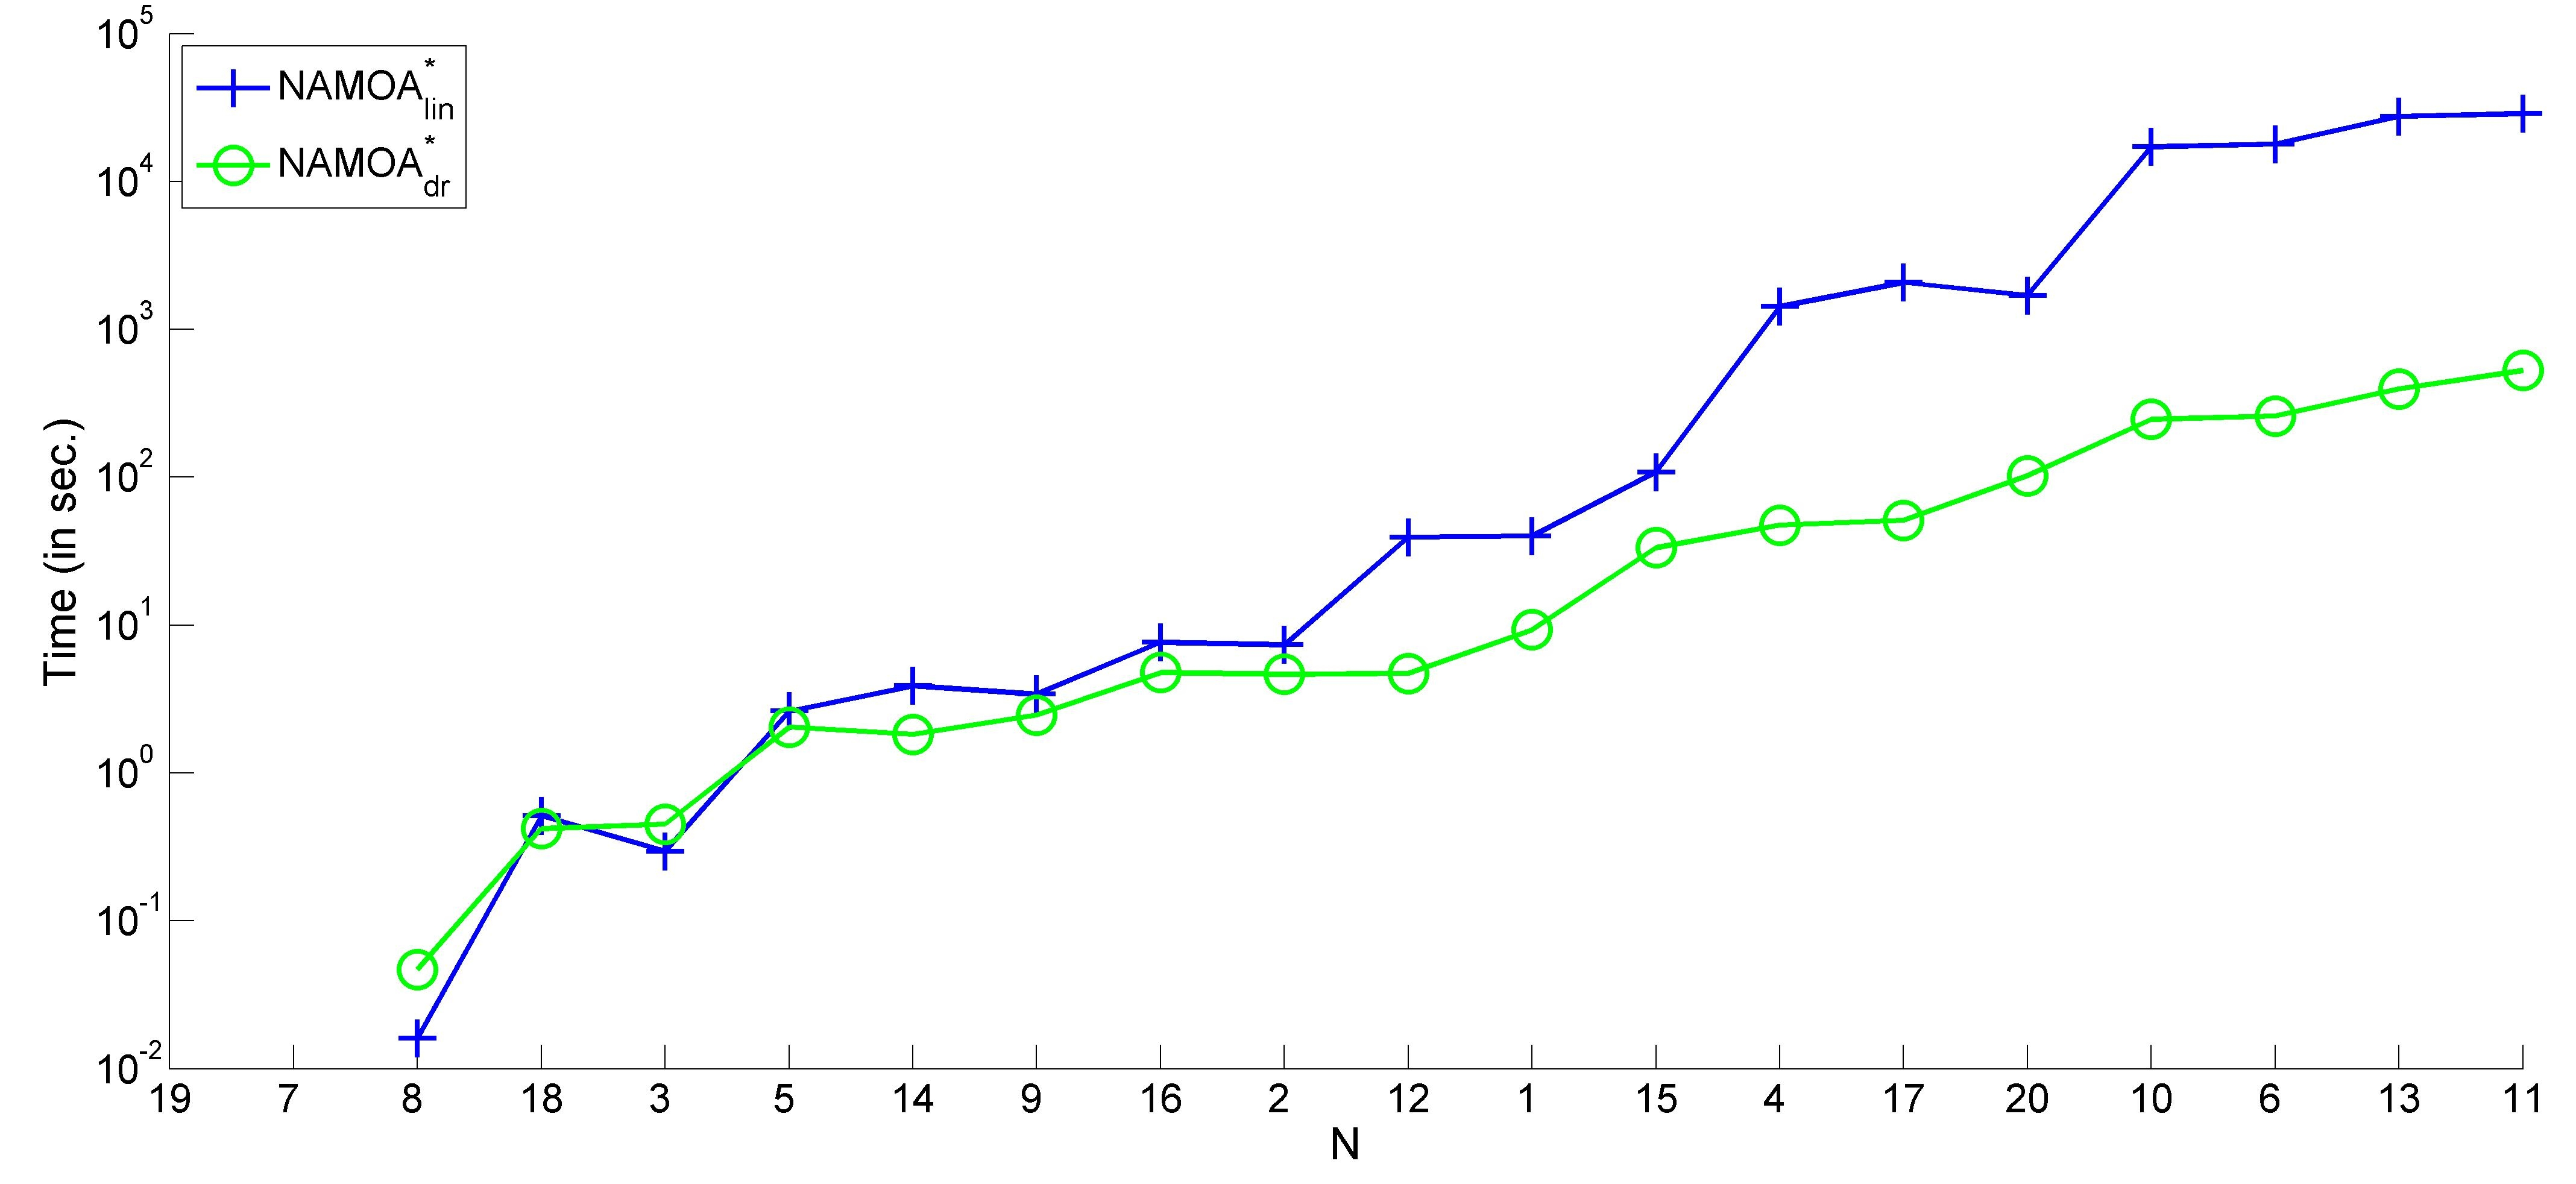
\includegraphics[scale=0.1]{figs/namoadr-roads-exe}
	\caption{Runtimes of \namoalin \ and \namoadr \ for Vermont map problems.}
	\end{figure}
\end{frame}
%%%%%%%%%%%%%%%%%%%%%%%%%%%%%%%%%%%%%%%%%%%%%%%%%%%%%%%%%%%%%%%%%%%%%%%%%%%%%%%%%%%%%%%%%%%%%%%%%%%%%%%%%
\begin{frame}<beamer:0>
\frametitle{\namoadr \ vs \namoa}
	\begin{table}
	\caption{Experimental summary for Vermont State map.}
		\vspace{2mm}
		\scalebox{1.2}{
		\begin{tabular}{ccccccc}
		\noalign{\smallskip} \hline \noalign{\smallskip}
		Map & $t_{\text{NAMOA}^* \text{lin}}$ & $t_{\text{NAMOA}^* \text{dr}}$ & \% \\
		\noalign{\smallskip} \hline \noalign{\smallskip}
		VT$_{cut}$ & 4,838.4 s. & \textcolor{ao}{84.6 s.} & \textcolor{red}{1.74} \\
		\noalign{\smallskip} \hline
		\end{tabular} 
		}
	\end{table}
\note{We see them first in this graphic, whenever the query becomes more time consuming, the advantage of the t-discarding version also grows. Moreover, in this table, the average runtime for \namoalin, the fastest previous version of \namoa, was 4 thousand and 8 hundred seconds, about 1 hour and 20 minutes, while \namoadr \ average runtime is less than one minute and a half.}
\end{frame}
%%%%%%%%%%%%%%%%%%%%%%%%%%%%%%%%%%%%%%%%%%%%%%%%%%%%%%%%%%%%%%%%%%%%%%%%%%%%%%%%%%%%%%%%%%%%%%%%%%%%%%%%%
\begin{frame}<beamer>[noframenumbering]
\frametitle{Empirical analyses}
	\begin{center}
		\LARGE{\textcolor{ao}{A posteriori \ vs \ A priori}}
	\end{center}
	\begin{table}
	\centering
	\scalebox{1.5}{
	\begin{tabular}{|lll|}
	\hline \noalign{\smallskip}
	\namoadr & vs & \lexgodr\\
	\noalign{\smallskip} \hline
	\end{tabular}
	}
	\end{table}
\note{}
\end{frame}
%%%%%%%%%%%%%%%%%%%%%%%%%%%%%%%%%%%%%%%%%%%%%%%%%%%%%%%%%%%%%%%%%%%%%%%%%%%%%%%%%%%%%%%%%%%%%%%%%%%%%%%%%
\begin{frame} 
\frametitle{\lexgodr \ vs \namoadr}
	\begin{table}
	\caption{Runtimes in seconds of \textcolor{ao}{\lexgodr} \ and \textcolor{red}{\namoadr} in Vermont State map problems.}
	\vspace{2mm}
	\centering
	\begin{tabular}{rrrrrrr}
	\hline \noalign{\smallskip}
	 & \multicolumn{5}{c}{\lexgodr} \\
	\noalign{\smallskip} \cline{2-6} \noalign{\smallskip}
	\namoadr & 1 & 0.75 & 0.5 & 0.25 & 0 & \multicolumn{1}{c}{$k_1$}\\
	\noalign{\smallskip} 
	\cline{1-6} \noalign{\smallskip} 
	84.66 & \textcolor{red}{94.89} & \textcolor{ao}{83.59} & \textcolor{ao}{57.38} & \textcolor{red}{157.02} & \textcolor{ao}{0.03} \\
	\hline
	\end{tabular}
	\end{table} 
\note{and the final comparison between the two best algorithmic alternatives gives us better results for \namoadr \ than we achieved in random grids, and the particular case here with 0.25. Even though the number of labels expanded is greatly reduced, t-discarding cannot be applied in that case, and therefore, \lexgodr \ runtime is almost two times slower.}
\end{frame}
%%%%%%%%%%%%%%%%%%%%%%%%%%%%%%%%%%%%%%%%%%%%%%%%%%%%%%%%%%%%%%%%%%%%%%%%%%%%%%%%%%%%%%%%%%%%%%%%%%%%%%%%%
\begin{frame} 
\frametitle{Empirical analyses}
\begin{center}
\Huge Why do the new algorithms have \textcolor{ao}{such a runtime performance}?
\end{center}
\end{frame}
%%%%%%%%%%%%%%%%%%%%%%%%%%%%%%%%%%%%%%%%%%%%%%%%%%%%%%%%%%%%%%%%%%%%%%%%%%%%%%%%%%%%%%%%%%%%%%%%%%%%%%%%%
\begin{frame} 
\frametitle{\lexgo \ vs \namoa}
	\begin{figure}
    	\centering
		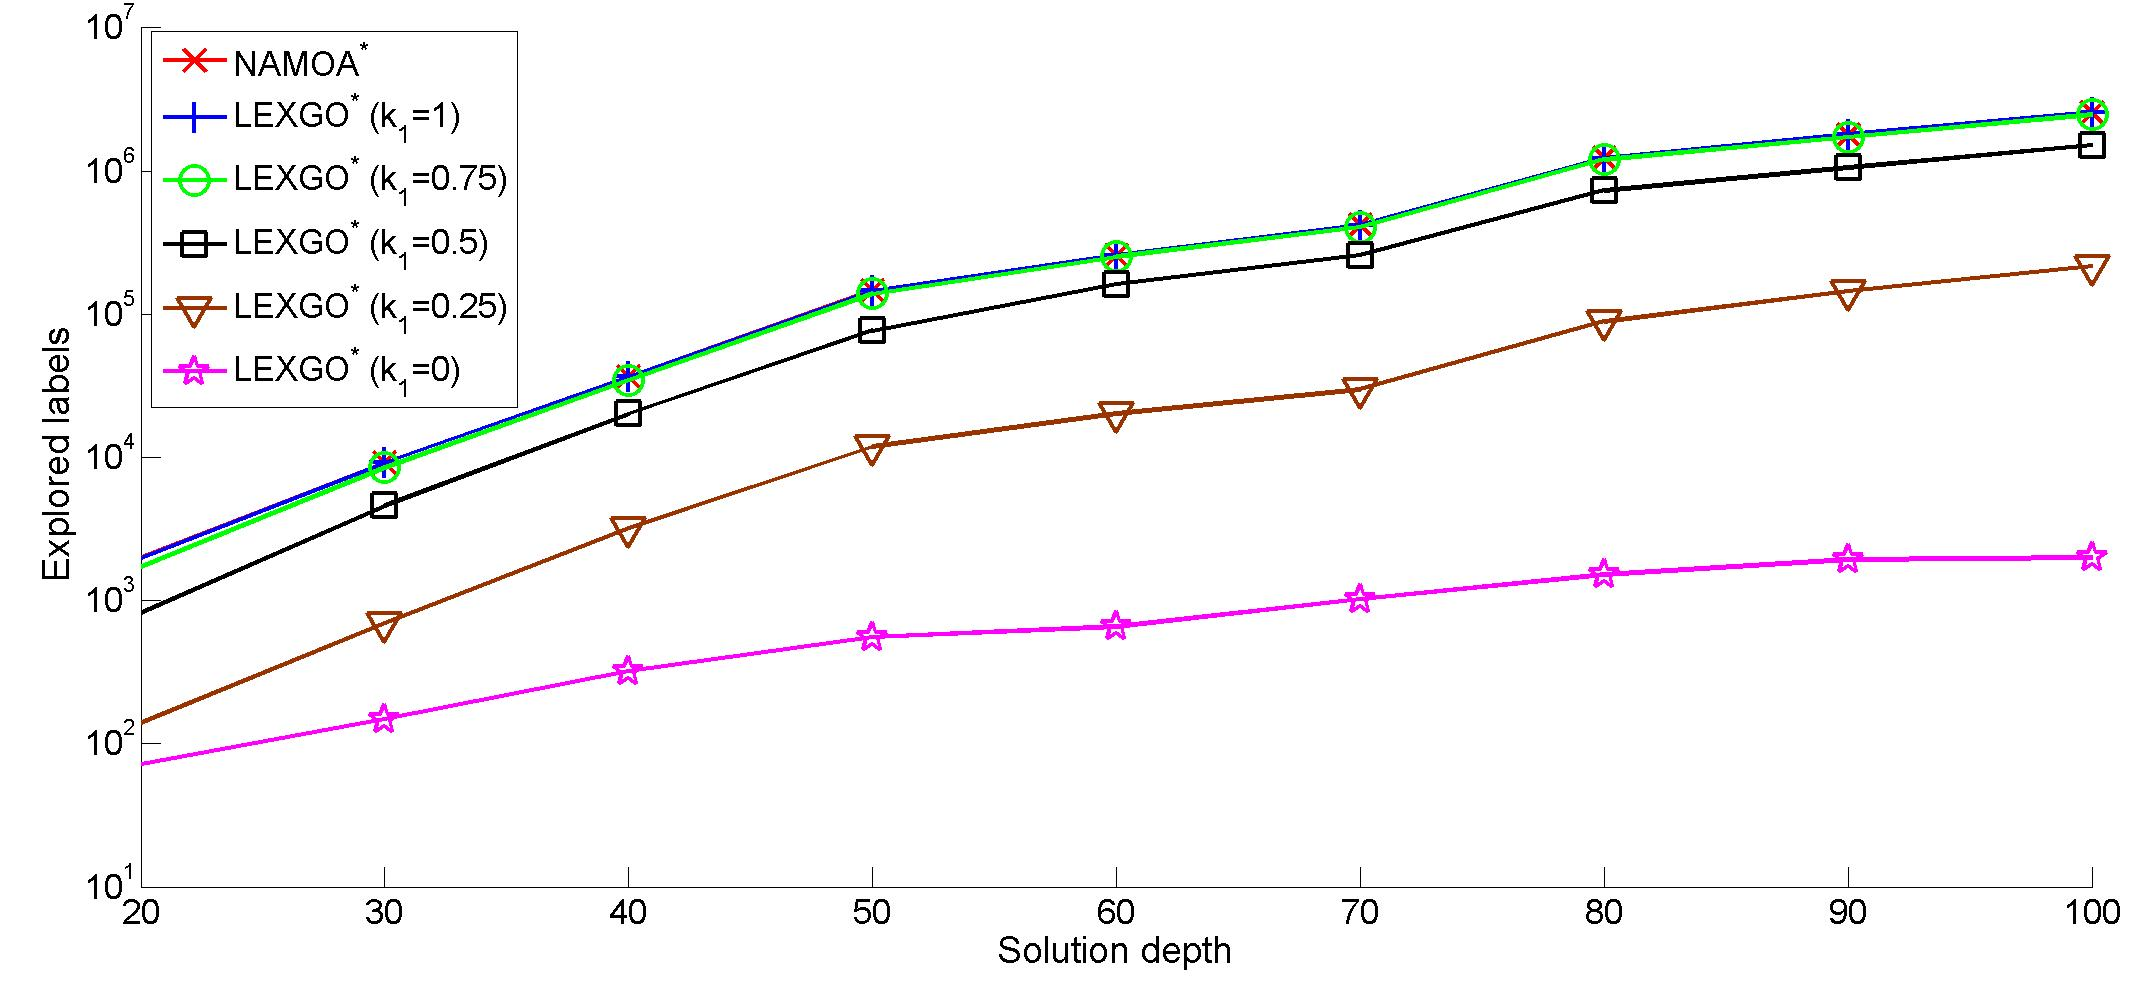
\includegraphics[scale=0.16]{figs/lexgo-labels}
		\caption{Explored labels by \namoa \ and \lexgo \ in grids.}
	\end{figure}
\note{We can observe a reduction of expanded labels of several orders of magnitude for \lexgo \ when k1 is equal to 0 or 0.25. The more restrictive the goals are the greater is that reduction. We can also observe that in the second class of experiments when the second level gets more restrictive.}
\end{frame}
%%%%%%%%%%%%%%%%%%%%%%%%%%%%%%%%%%%%%%%%%%%%%%%%%%%%%%%%%%%%%%%%%%%%%%%%%%%%%%%%%%%%%%%%%%%%%%%%%%%%%%%%%
\begin{frame} 
\frametitle{Deviation-based pruning}
	\begin{figure}
    	\centering
		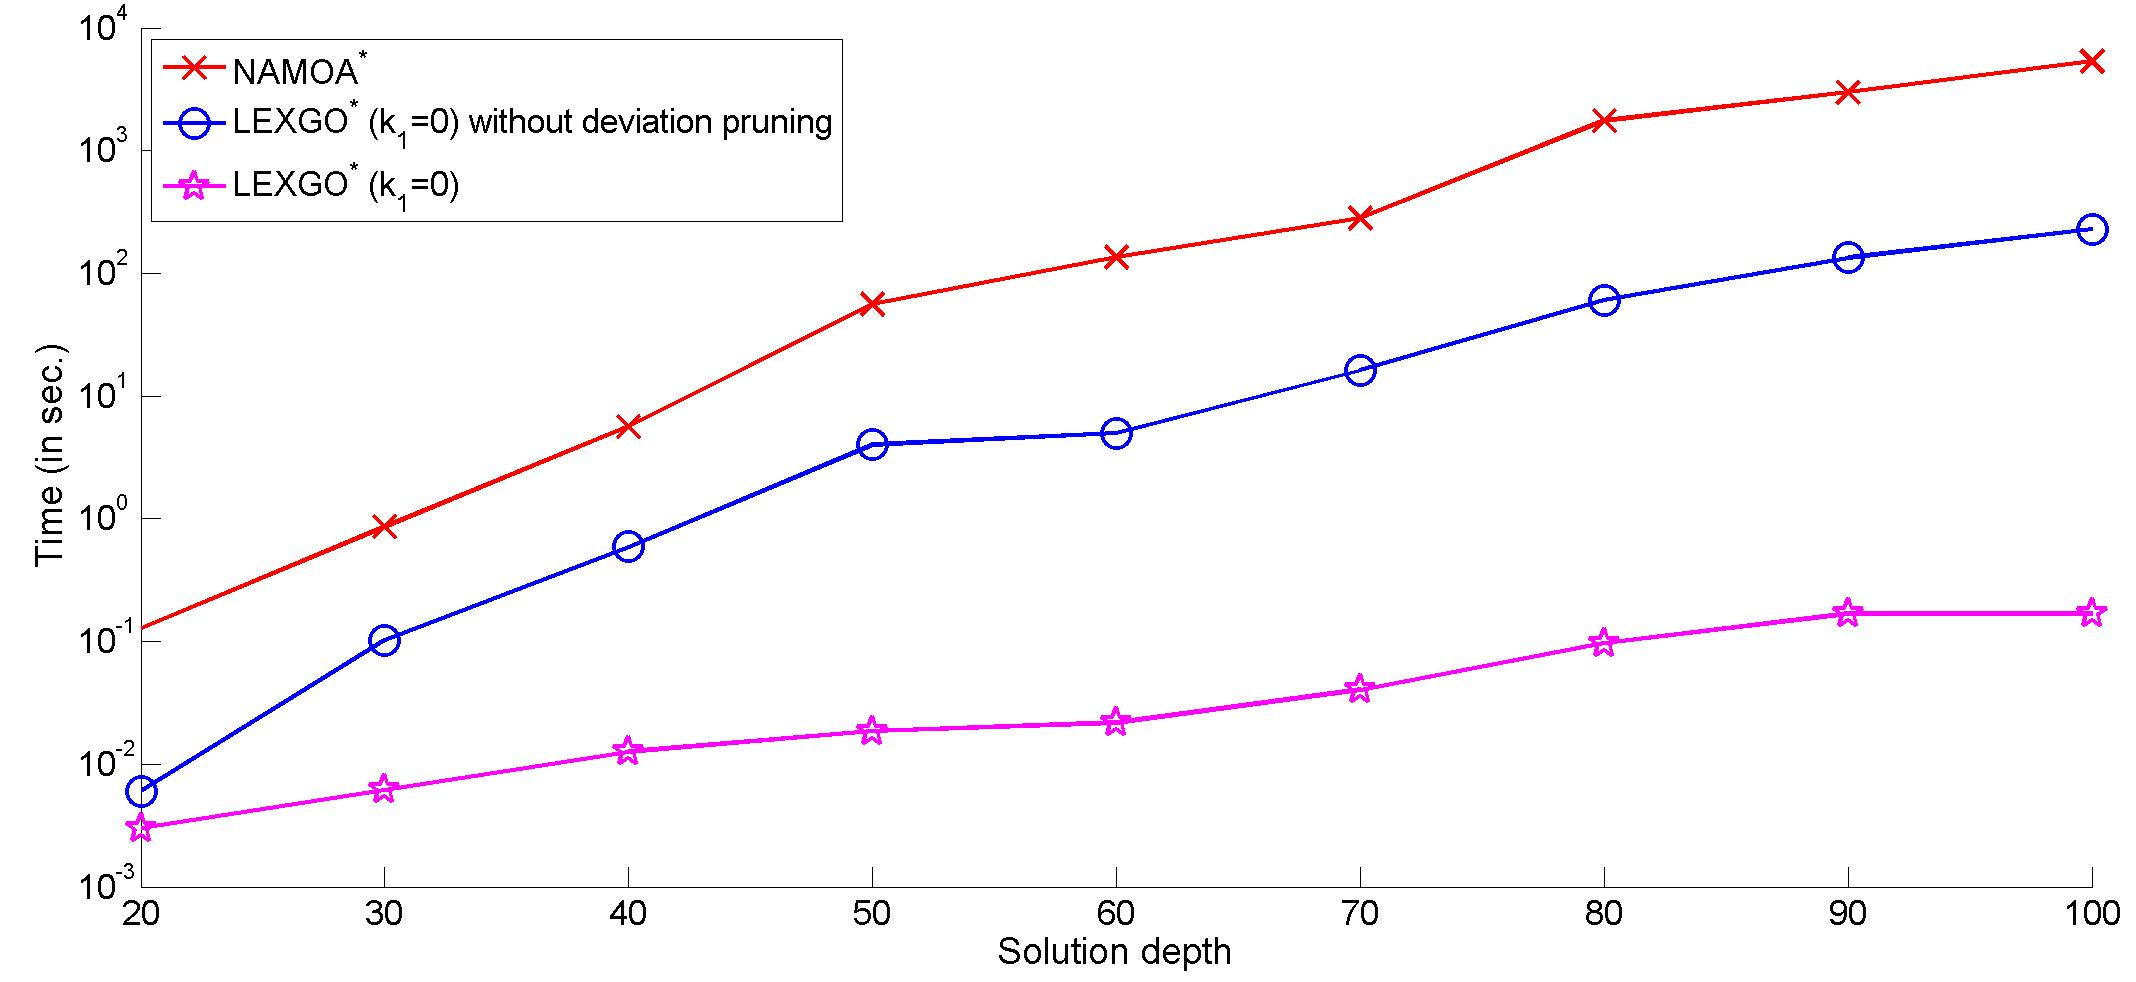
\includegraphics[scale=0.16]{figs/lexgo-dev-pruning}
	\caption{Impact of deviation pruning in $k_1 = 0$ experiments.}
	\end{figure}
\note{In this graphic we see the runtimes of \namoa \ and \lexgo \ with goals in the ideal point with and without using the deviation-based pruning. For the most difficult problems, the runtimes without this rule vary from minutes to tenths of a second.}
\end{frame}
%%%%%%%%%%%%%%%%%%%%%%%%%%%%%%%%%%%%%%%%%%%%%%%%%%%%%%%%%%%%%%%%%%%%%%%%%%%%%%%%%%%%%%%%%%%%%%%%%%%%%%%%%
\begin{frame} 
\frametitle{\namoadr \ vs \namoa}
	\begin{table}
	\caption{Set sizes for Vermont State map.}
		\vspace{2mm}
		\scalebox{1.2}{
		\begin{tabular}{ccc}
		\hline \noalign{\smallskip}
		Map & $(\frac{\sum T(G_{cl})}{\sum G_{cl}})$\% & $(\frac{\sum T(C^*)}{\sum C^*})$\% \\
		\noalign{\smallskip} \hline \noalign{\smallskip} 
VT$_{cut}$ & \textcolor{red}{3.43} & \textcolor{red}{2.45} \\
		\noalign{\smallskip} \hline
		\end{tabular} 
		}
	\end{table}
\note{The relative size of the truncated sets is also reduced to 2 to 3\% of the size of the standard sets Gcl and COSTS.}
\end{frame}
%%%%%%%%%%%%%%%%%%%%%%%%%%%%%%%%%%%%%%%%%%%%%%%%%%%%%%%%%%%%%%%%%%%%%%%%%%%%%%%%%%%%%%%%%%%%%%%%%%%%%%%%%
\begin{frame}
\frametitle{\namoadr \ vs \namoa}
	\begin{figure}
    	\centering
		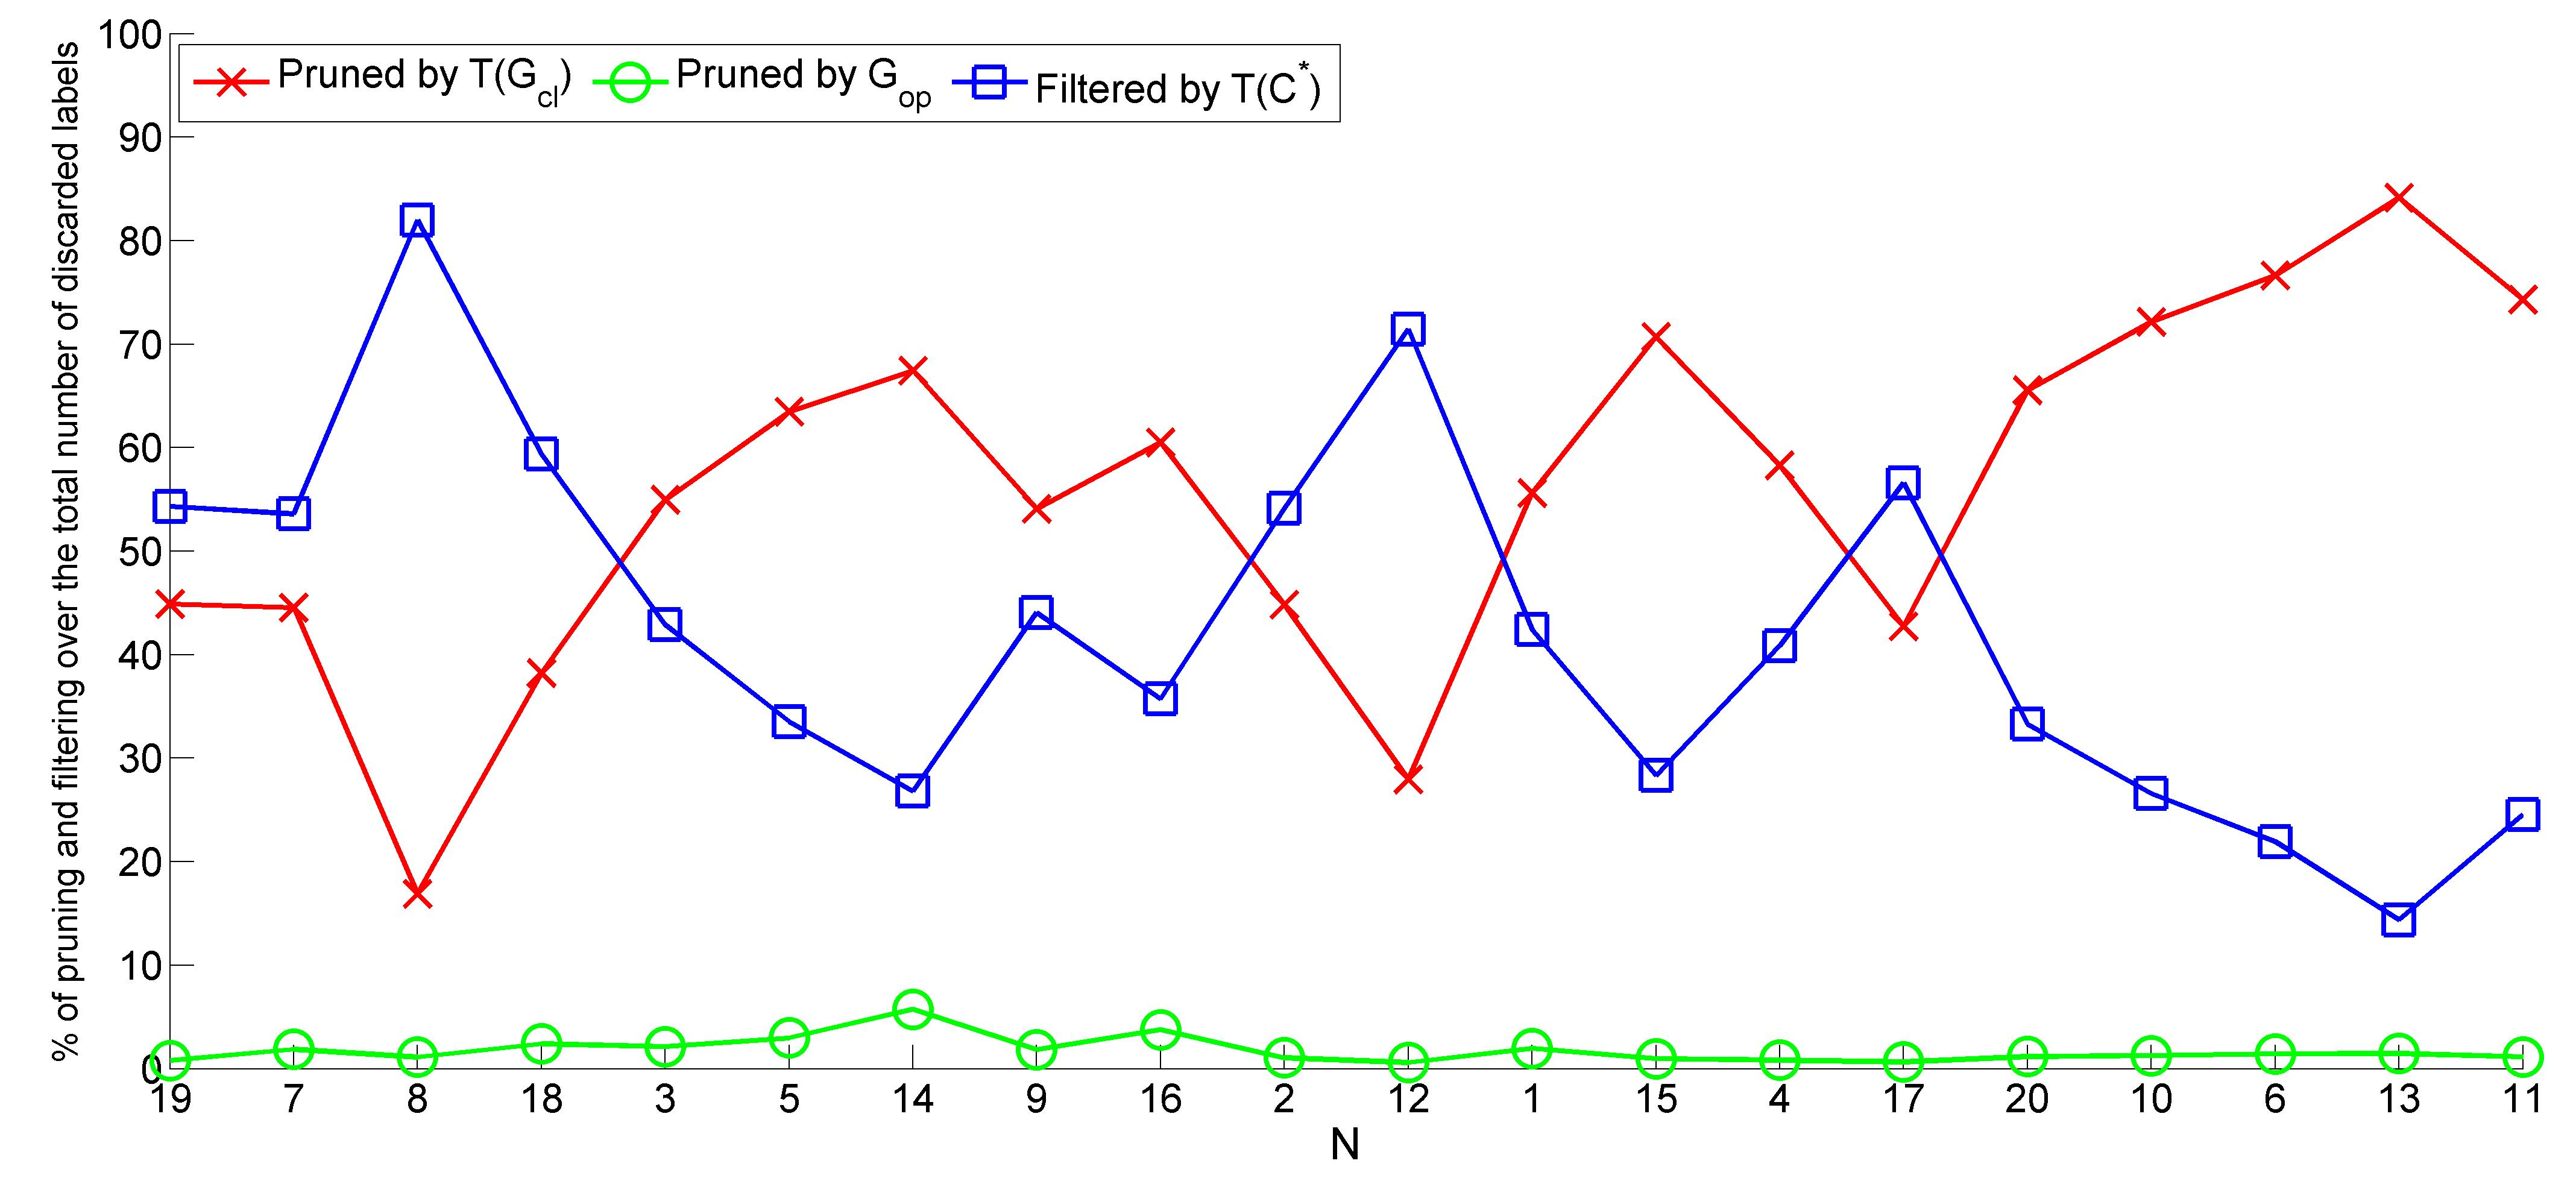
\includegraphics[scale=0.08]{figs/pruned-filtered-vermont}
	\caption{Discarded labels in Vermont problems.}
	\end{figure}
\note{The percentage of labels pruned by Gop is even smaller for road maps, so that, we can expect even bigger runtime improvements in this domain.}
\end{frame}
%%%%%%%%%%%%%%%%%%%%%%%%%%%%%%%%%%%%%%%%%%%%%%%%%%%%%%%%%%%%%%%%%%%%%%%%%%%%%%%%%%%%%%%%%%%%%%%%%%%%%%%%%
\begin{frame} 
\frametitle{New York experiments}
	\LARGE{Now, we can even solve \textcolor{red}{more} problems!}
	\vspace{5mm}
	\begin{table}
	\centering
	\scalebox{1}{
	\begin{tabular}{crr}
	\hline \noalign{\smallskip}
	Problem \# & \namoadr & \namoalin \\
	\noalign{\smallskip} \hline \noalign{\smallskip}
	\#11 & \textcolor{red}{30 min.} & 31 hours \\
	\noalign{\smallskip} \hline \noalign{\smallskip}
	\#6 & \textcolor{red}{3 hours} & 25 days \\
	\noalign{\smallskip} \hline
	\end{tabular}
	}
	\end{table}
\note{As an example, we are going to show now the runtimes of \namoadr \ and \namoalin \ sorted by increasing difficulty. The easiest problem of New York was solved by both algorithms really fast. The second problem was solved by \namoadr \ twice as fast as \namoalin. The third problem, number 16, was solved around 6 times faster. The fourth problem was solved by \namoadr \ in two minutes and half and more than an hour by the standard version of \namoa. The fifth problem by difficulty was solved by \namoadr \ in less than half an hour, and it tood 31 hours to be solved by \namoalin, in other words, a speed up of more than sixty. Problem six, was solved in about three hours by \namoadr \ and the impressive amount of 25 days by \namoalin. We can easily see where this is going if we wanted to keep solving problems with \namoalin.}
\end{frame}
%%%%%%%%%%%%%%%%%%%%%%%%%%%%%%%%%%%%%%%%%%%%%%%%%%%%%%%%%%%%%%%%%%%%%%%%%%%%%%%%%%%%%%%%%%%%%%%%%%%%%%%%%


% Conclusions
% -----------------------------------------------------------------------------
%---------------------------------------------------------------------
%
%                          conclusions.tex
%
%---------------------------------------------------------------------
%
% conclusions.tex
% Copyright 2015 Dr. Francisco J. Pulido
%
% This presentation belongs to the PhD titled "New Techniques and Algorithms for Multiobjective and Lexicographic Goal-Based Shortest Path Problems", distributed under the Creative Commons Licence Attribution-NonCommercial-NoDerivs 3.0, available in http://creativecommons.org/licenses/by-nc-nd/3.0/. The complete PhD dissertation is freely accessible from http://www.lcc.uma.es/~francis/

\section{Conclusions \& future work}

\subsection{Conclusions}
\begin{frame} 
\frametitle{Conclusions}
	\begin{enumerate}
		\item We have tackled the \textcolor{ao}{MSP with lexicographic preferences} from two approaches: \textcolor{ao}{a priori} and \textcolor{ao}{a posteriori}.
		\item On the a priori approach, we have contributed two new algorithms: \textcolor{ao}{\lexgo} \ and \textcolor{ao}{\lexgodr}. 
		\item On the a posteriori approach: \textcolor{ao}{\namoadr} \ based on \namoa.
		\item All algorithmic approaches have been \textcolor{ao}{formally proved to be admissible}.
		\item The contributions of this thesis \textcolor{ao}{outperform the state of the art} in \textcolor{red}{an order of magnitude} for medium size problems and \textcolor{red}{two orders of magnitude} for the hardest problems. 
		\item \textcolor{ao}{\namoadr} \ \textcolor{ao}{\lexgodr} represent \textcolor{ao}{the new state of the art} in \textcolor{ao}{MSP with lexicographic goals}.
	\end{enumerate}
\note{}
\end{frame}

\subsection{Future work}
\begin{frame} 
\frametitle{Future work}
	\begin{enumerate}
		\item Investigate more \textcolor{ao}{formal proofs about \lexgo}, concerning the optimality in its class of algorithms and the expansion of labels when using more informed lower bounds.
		\vspace{3mm}
		\item Extend \lexgo \ to be used with \textcolor{ao}{other GP models} or \textcolor{ao}{other formulas to measure the deviation} from goals. 
		\vspace{3mm}
		\item \textcolor{ao}{Research the applicability} of t-discarding to other multiobjective or multicriteria search algorithms with lower bounds.
		%\item Tighten the concept of dominance for those cases where only a small amount of solutions are required.
		\vspace{3mm}
		\item Bring multicriteria search algorithms to \textcolor{ao}{real route planning applications.} 
	\end{enumerate}
\note{}
\end{frame}


\begin{frame}<beamer>[noframenumbering]
  \frametitle{}
  \begin{center}
    \Huge \textcolor{blue}{Thank you for your attention !!!}
    \Huge \textcolor{black}{Gracias por su atenci\'{o}n !!!}
  \end{center}
\end{frame}

\begin{frame}<beamer>[noframenumbering]
\titlepage
\end{frame}

\end{document}
